\documentclass{article}
\usepackage[a4paper,margin=3cm,footskip=.5cm]{geometry}
\usepackage{amsmath,amssymb,amsthm,amsfonts,mdframed,kotex}
\newcounter{problem}
\newcommand{\bp}
{\stepcounter{problem}\begin{mdframed}
[frametitle={\theproblem},skipabove=10pt,skipbelow=10pt]}
\newcommand{\ep}{\end{mdframed}}
\newcommand{\parall}{\mathbin{\!/\mkern-5mu/\!}}
\mdfsetup{nobreak=true}

\title{미리-03:최상위수학 2-2}
\date{\today}
\author{}

\begin{document}
\maketitle
\newpage
\bp
아래 그림은 정사각형들을 붙여 놓은 것이다.
정사각형 \(A\)의 한 변의 길이와 정사각형 \(B\)의 한 변의 길이의 비를 가장 간단한 자연수의 비로 나타내어라.
\par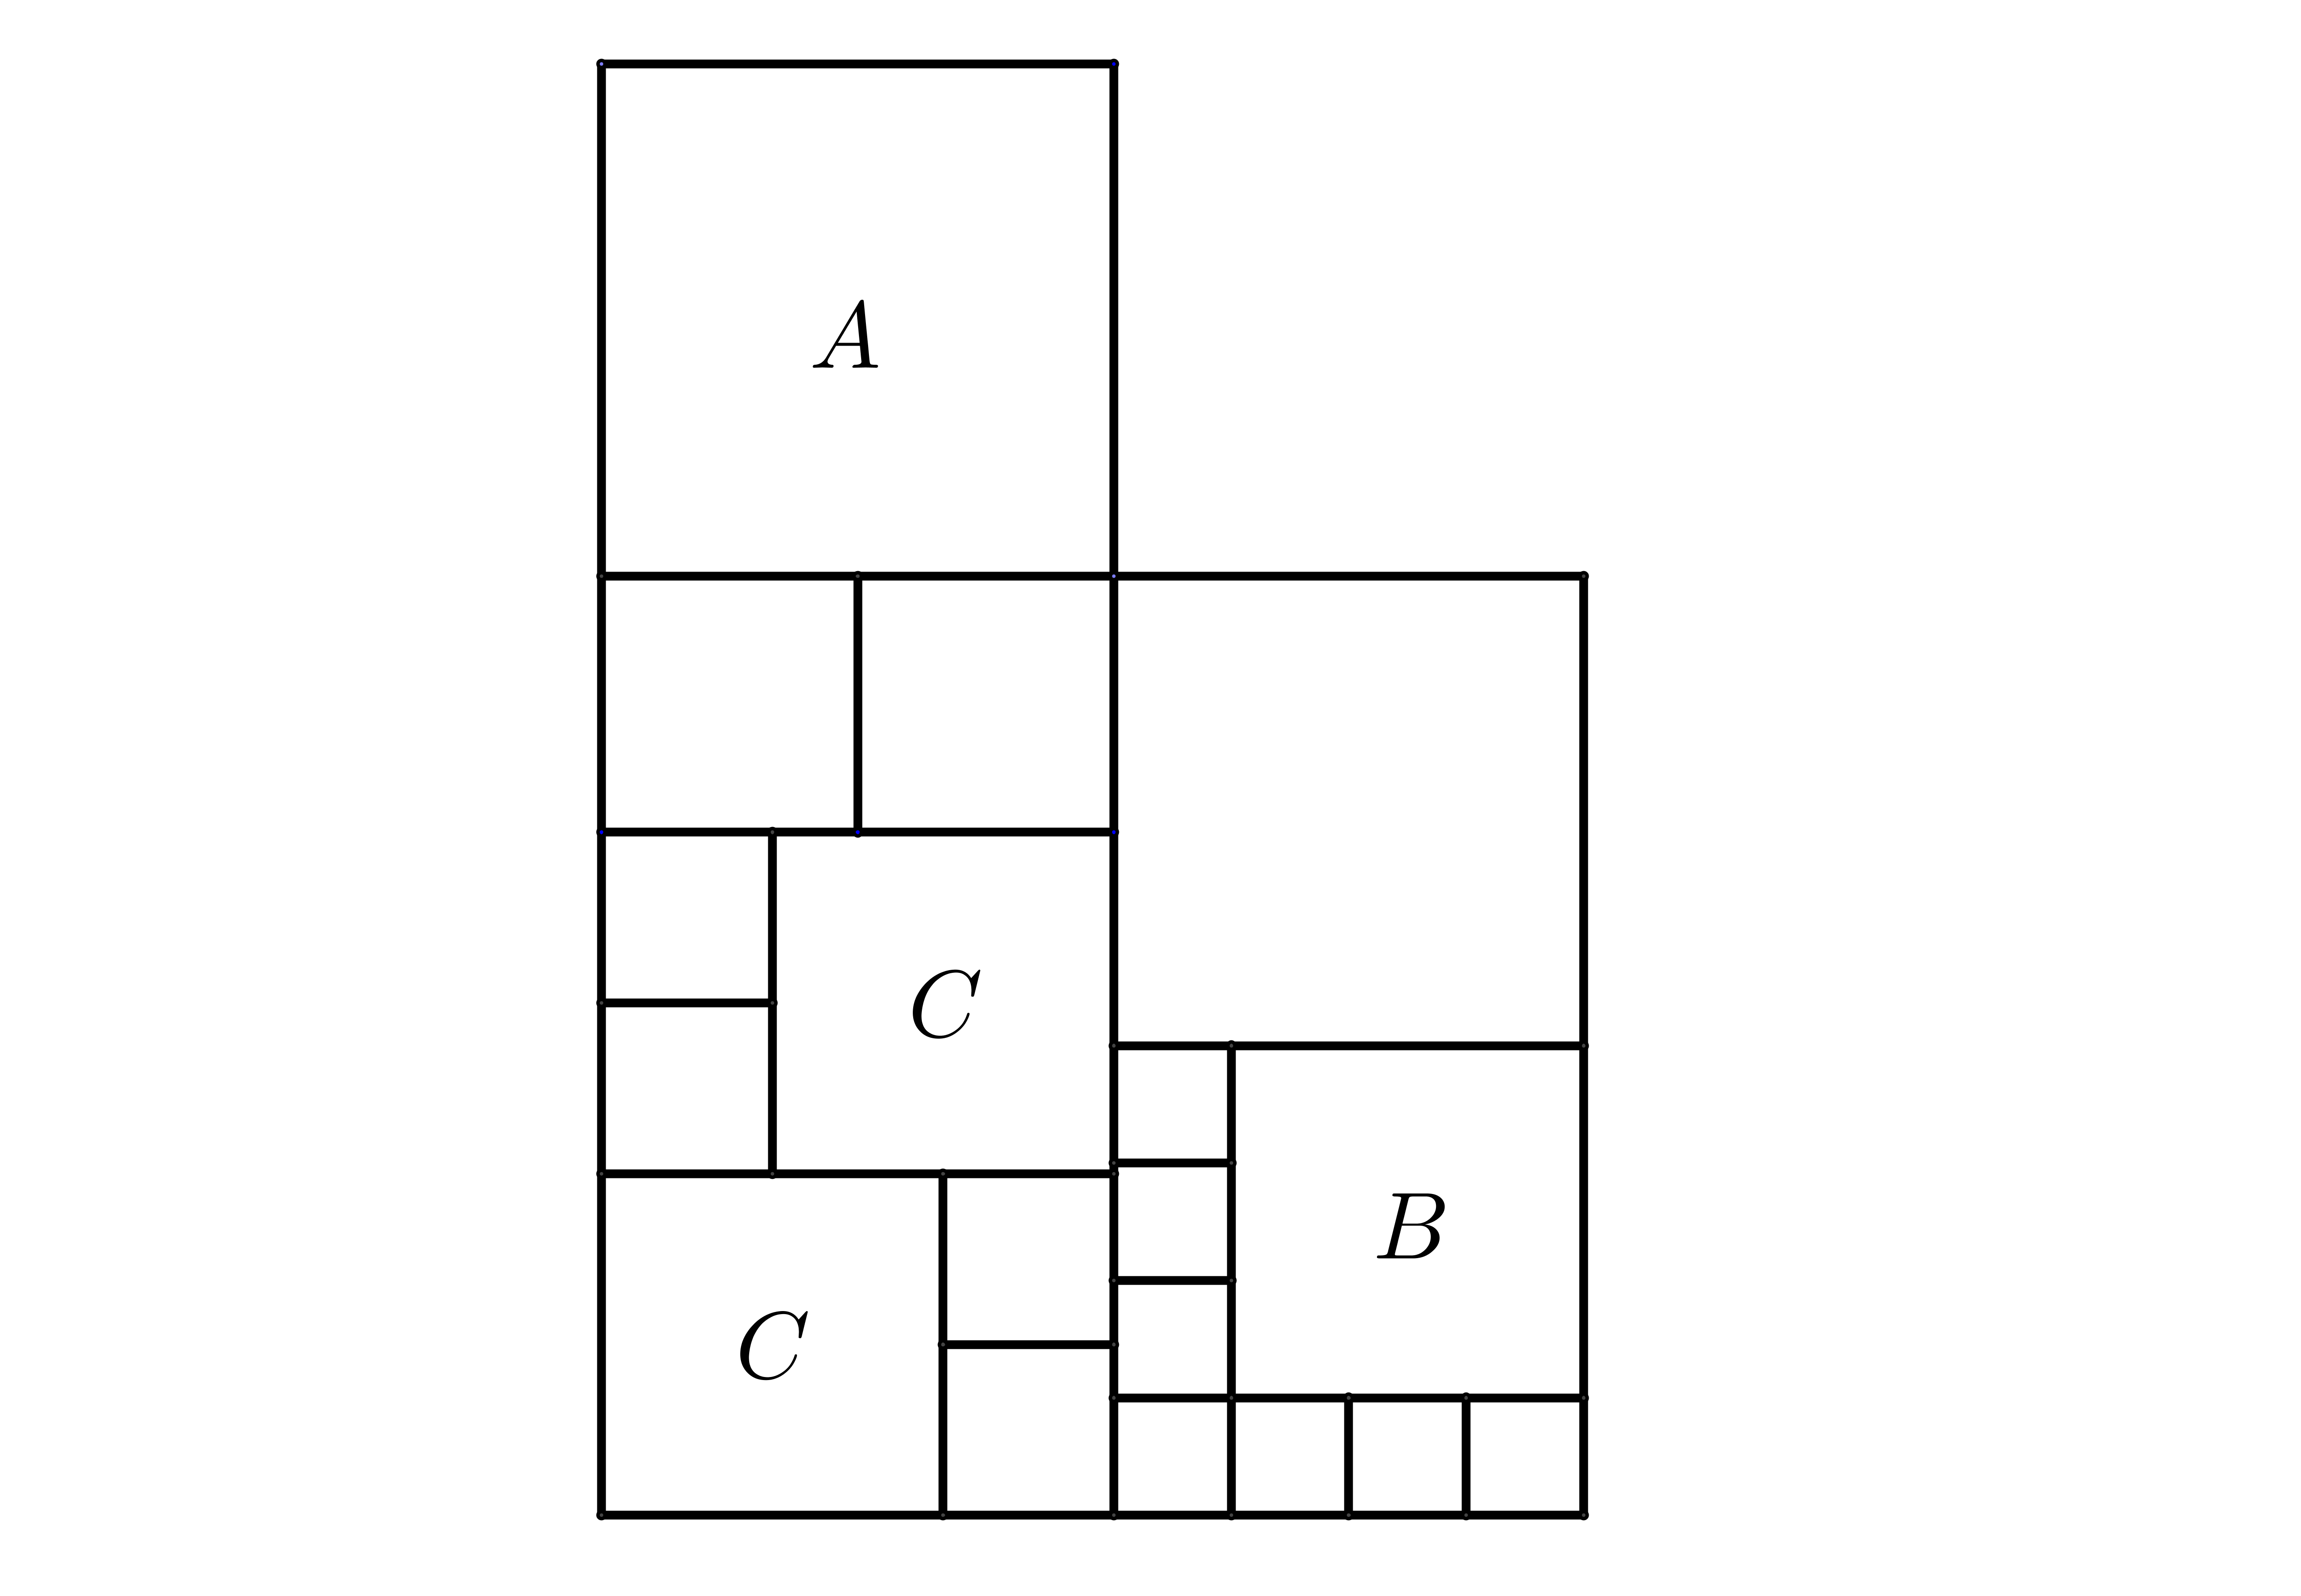
\includegraphics[width=0.4\textwidth]{top_math_p64_07}
\ep

\bp
\(AD=15\), \(BC=40\), \(AH=20\)이고 \(\square PQRS\)가 정사각형일 때, 이 정사각형의 한 변의 길이를 구하여라.
\par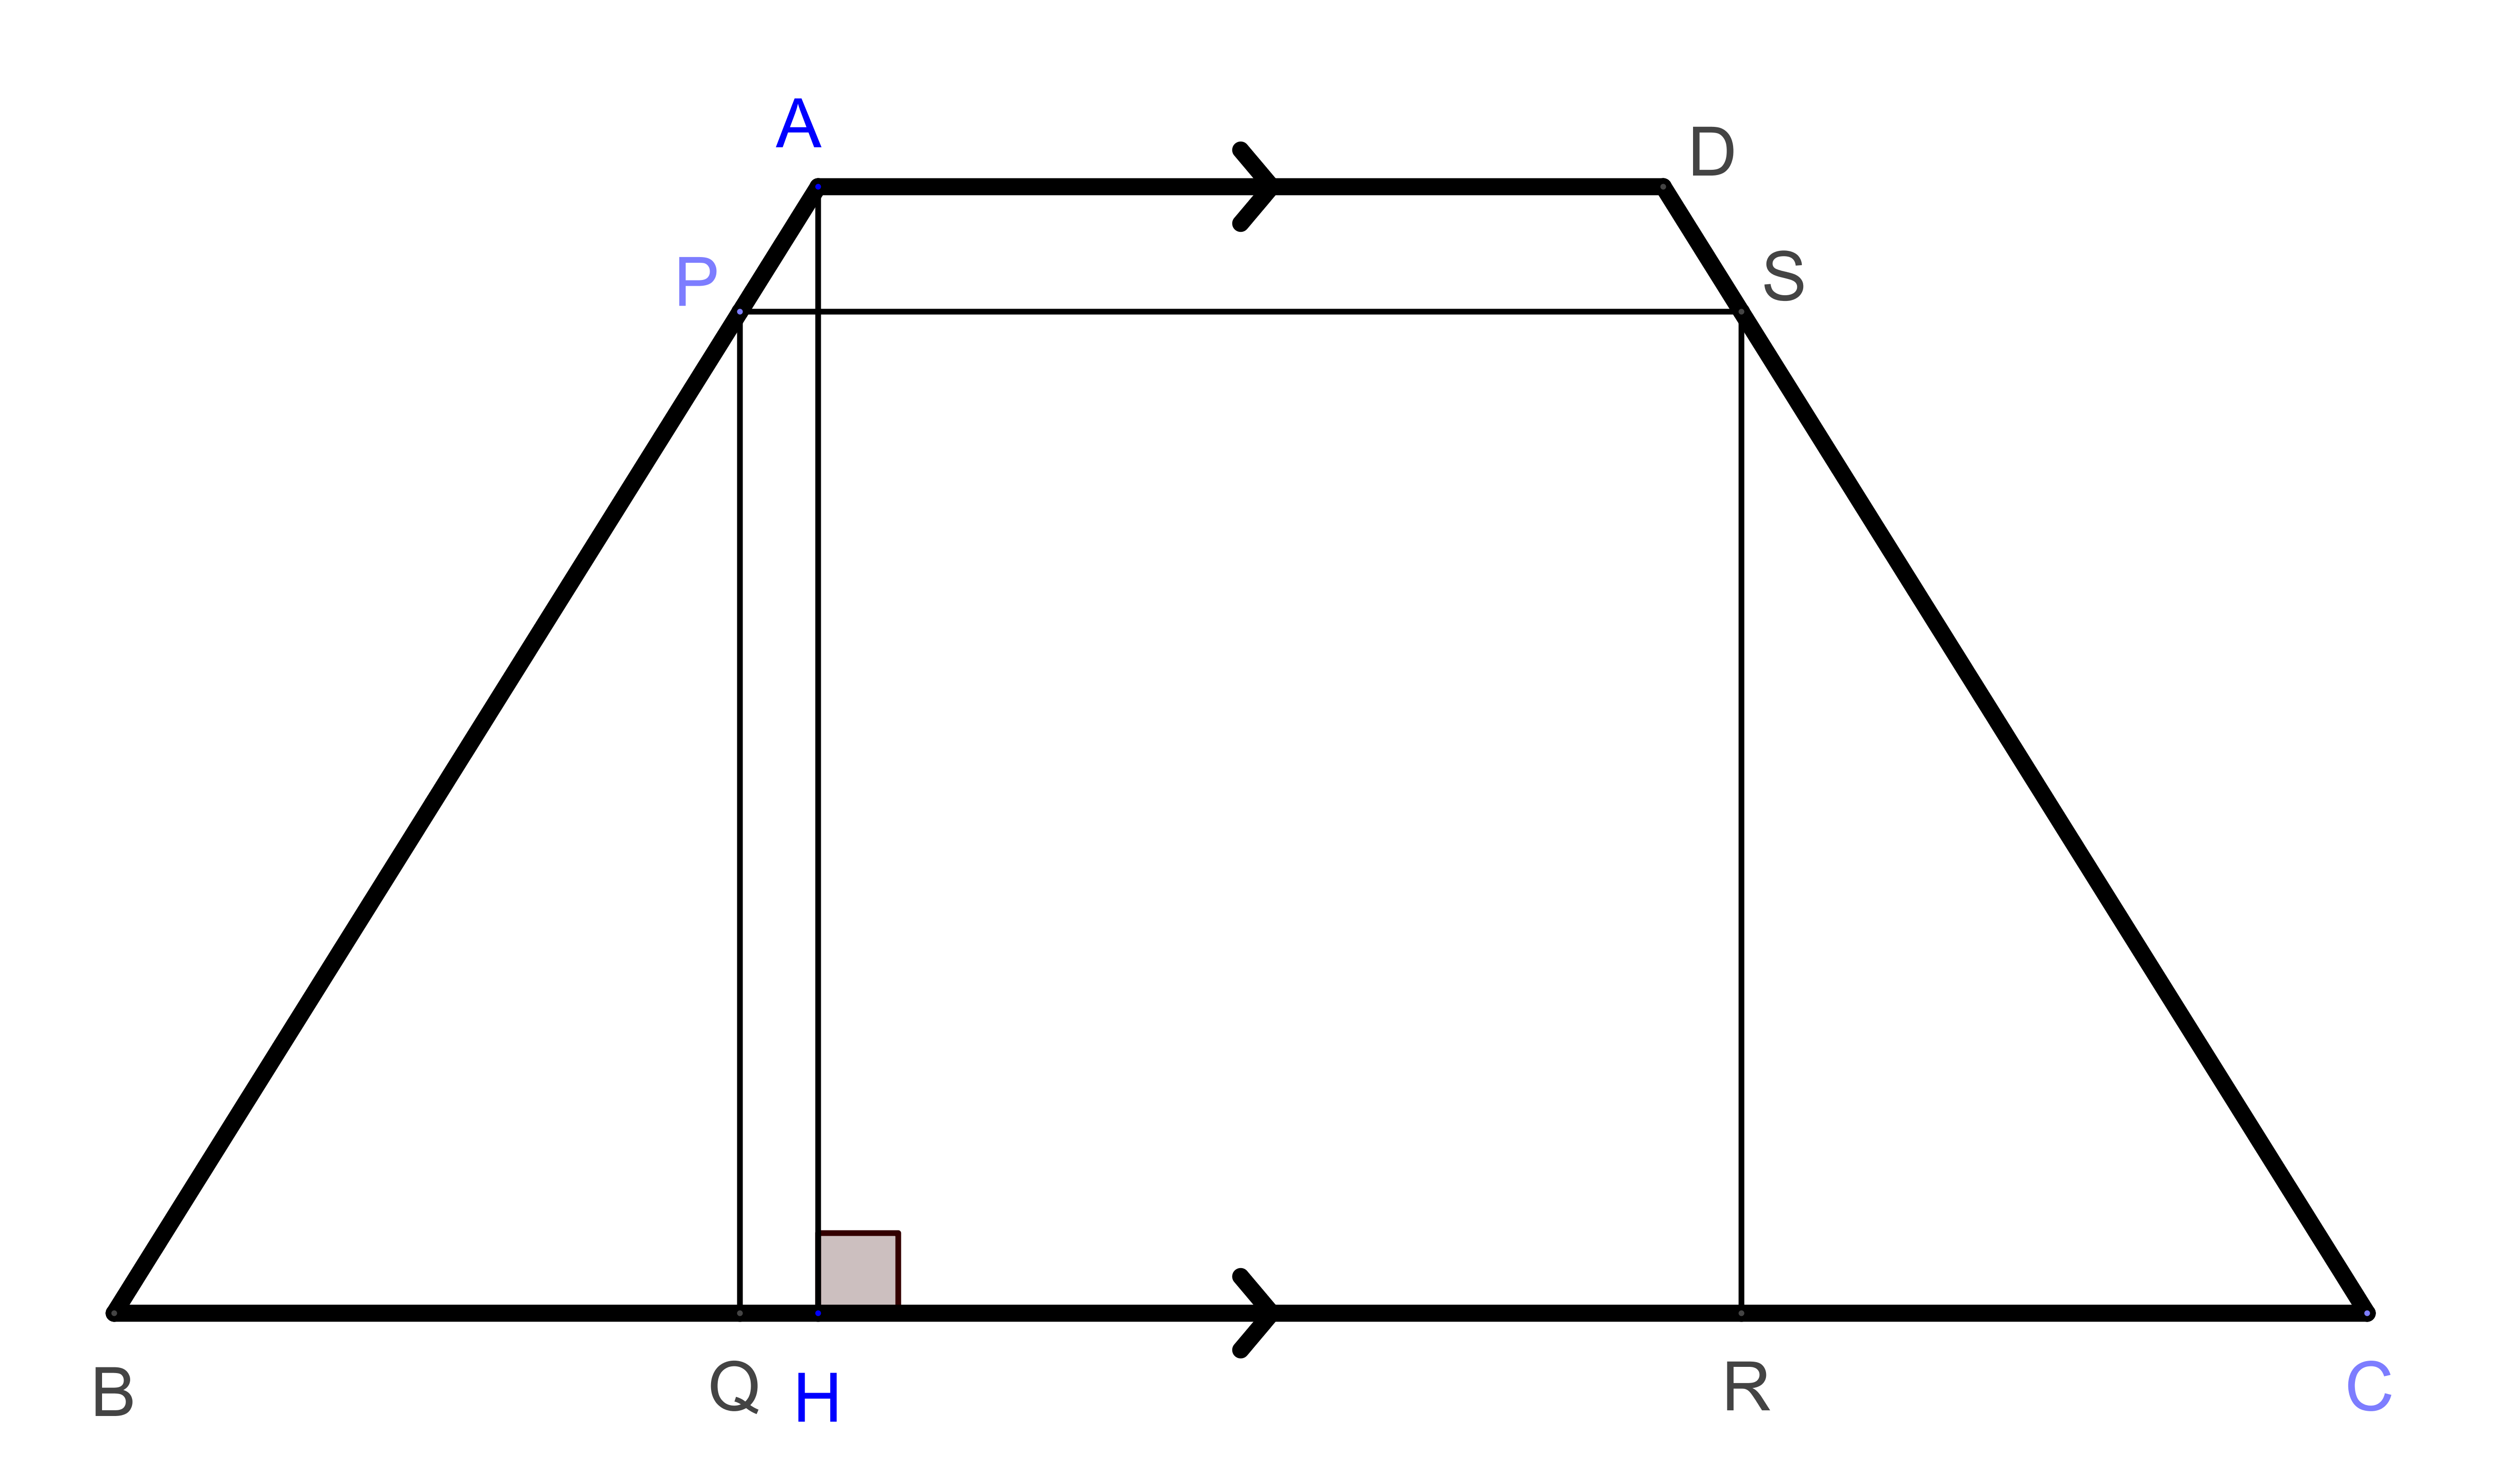
\includegraphics[width=0.5\textwidth]{top_math_p64_08}
\ep

\bp
직사각형 \(ABCD\) 내부의 점 \(P\)에 대해 \(\triangle PAB=9\). \(\triangle PBC=6\)일 때, \(\triangle PBD\)의 넓이를 구하여라.
\par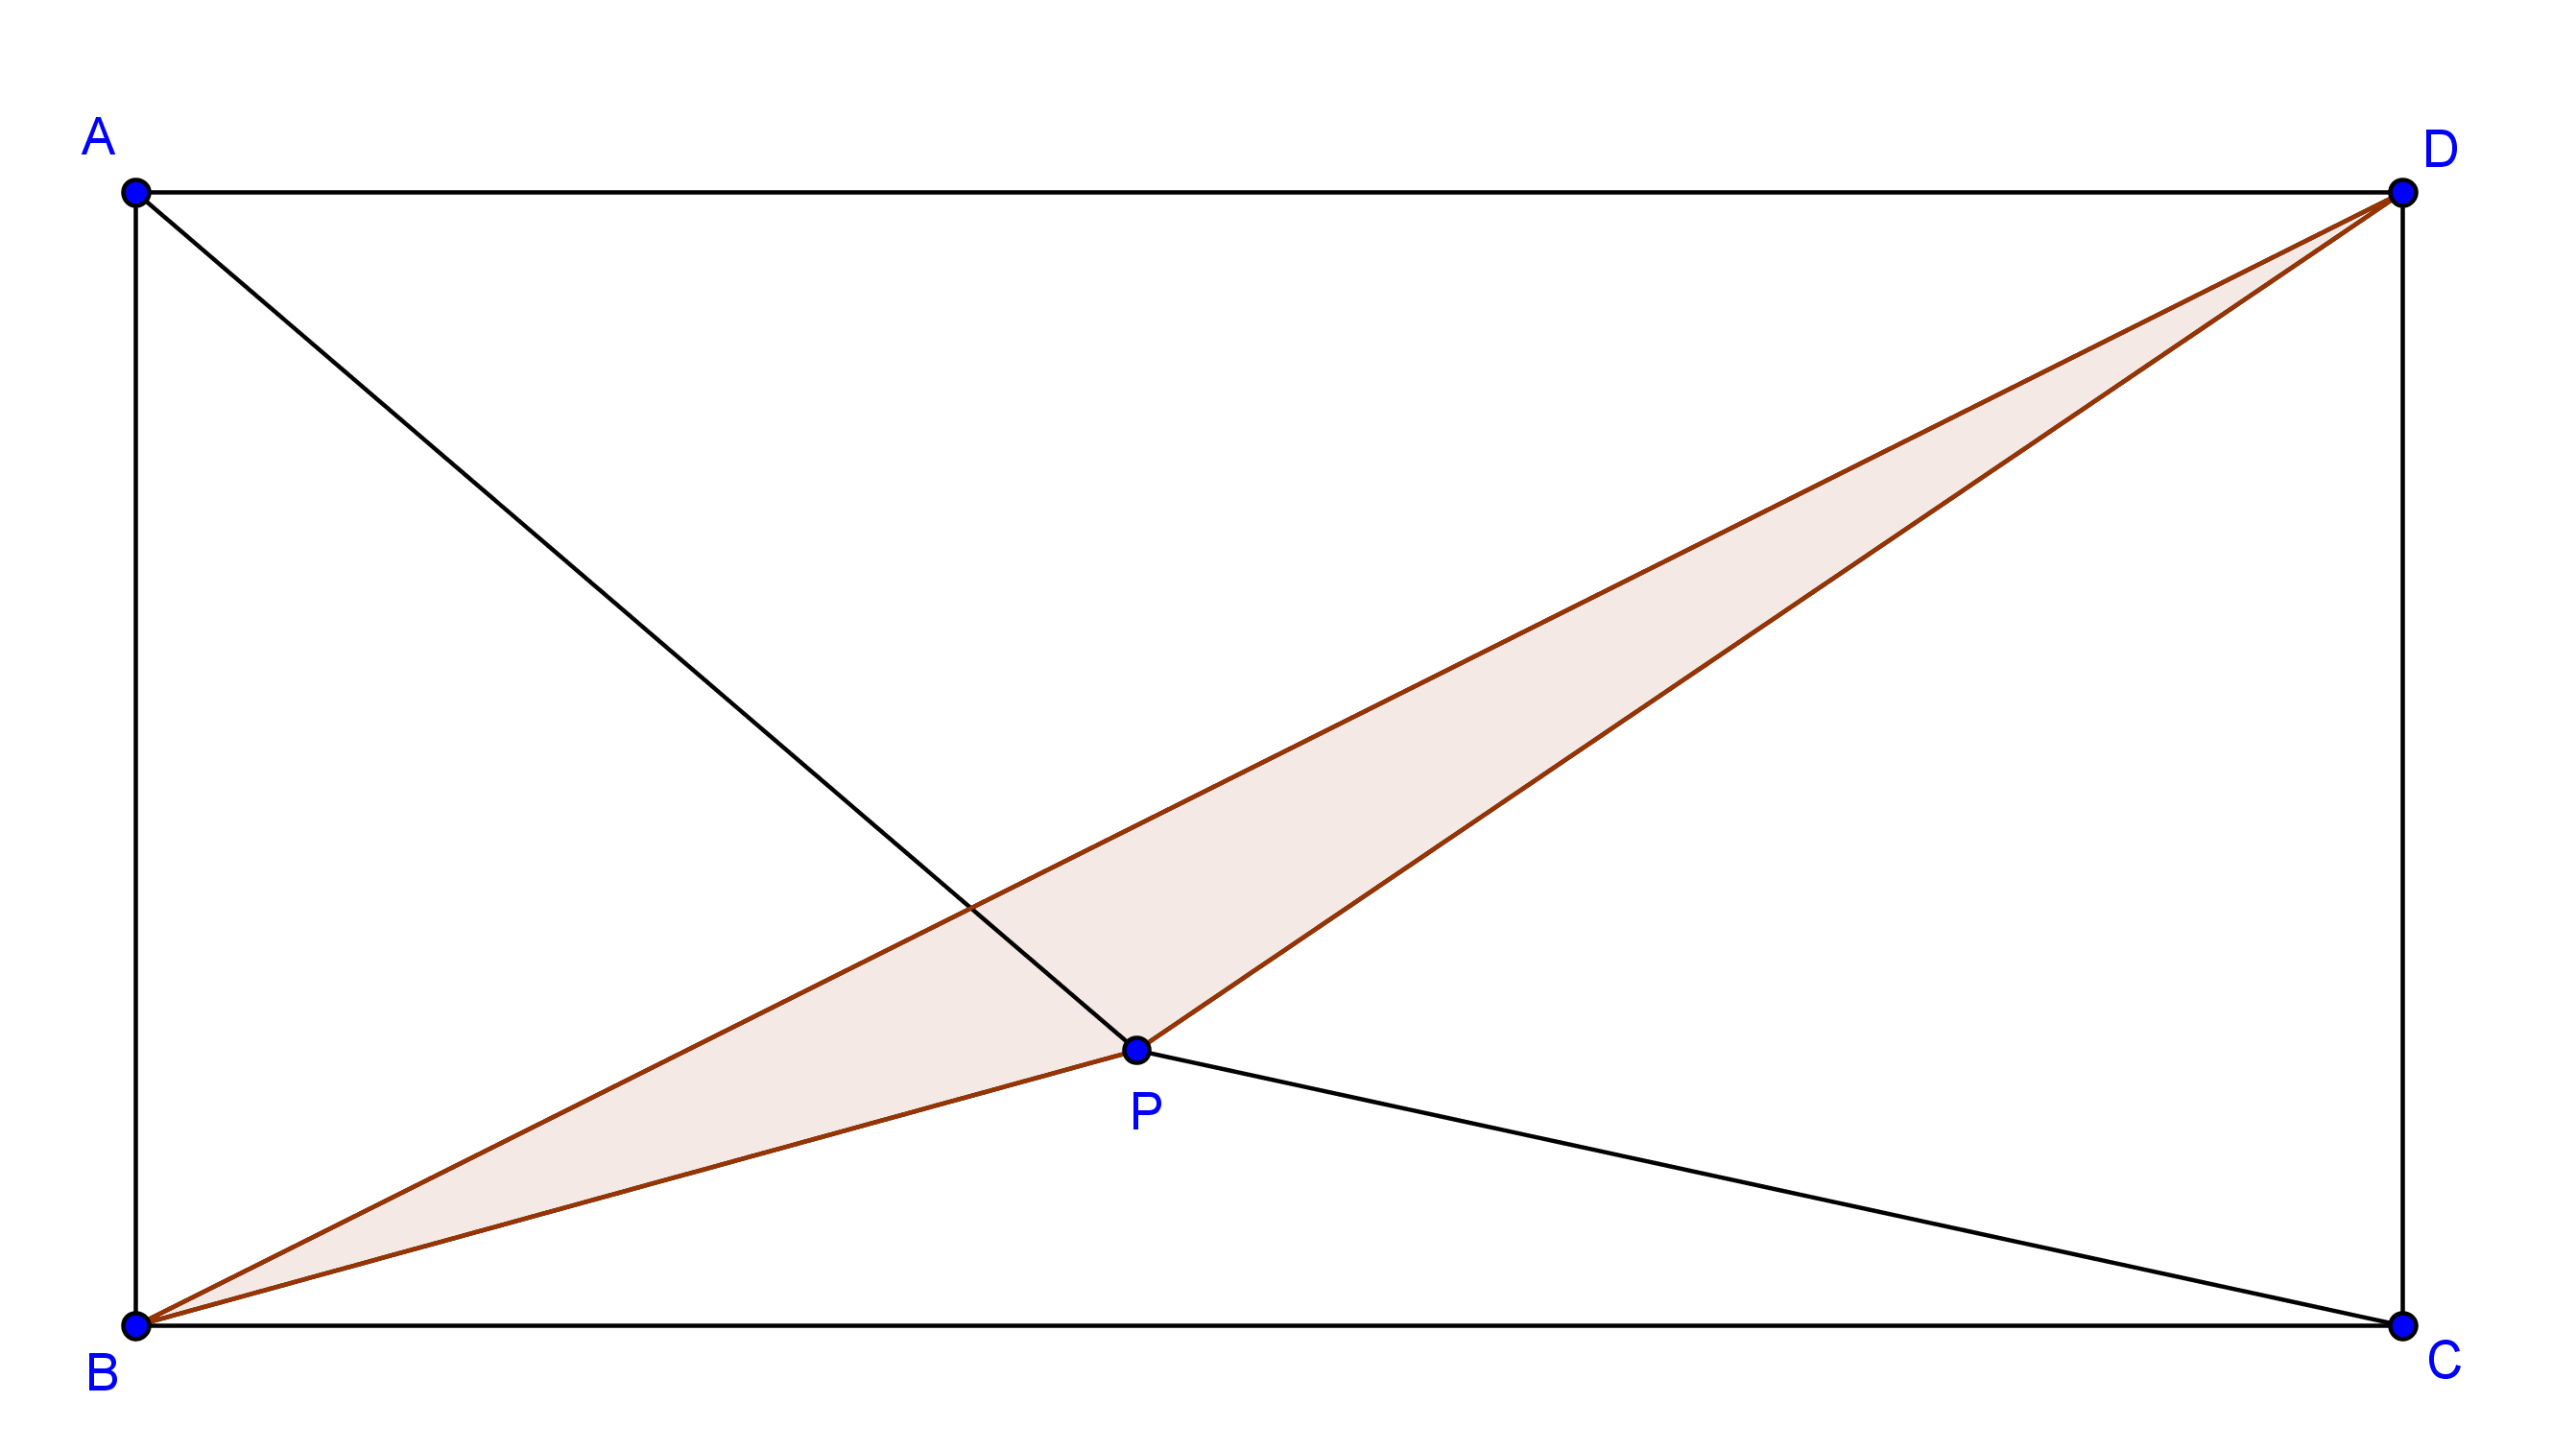
\includegraphics[width=0.5\textwidth]{top_math_p64_09}
\ep

\bp
아래 그림과 같이 직사각형 \(ABCD\)의 한 꼭지점 \(B\)를 \(CD\)의 중점 \(M\)에 오도록 접었을 때 \(BP:PC\)를 구하여라.
\par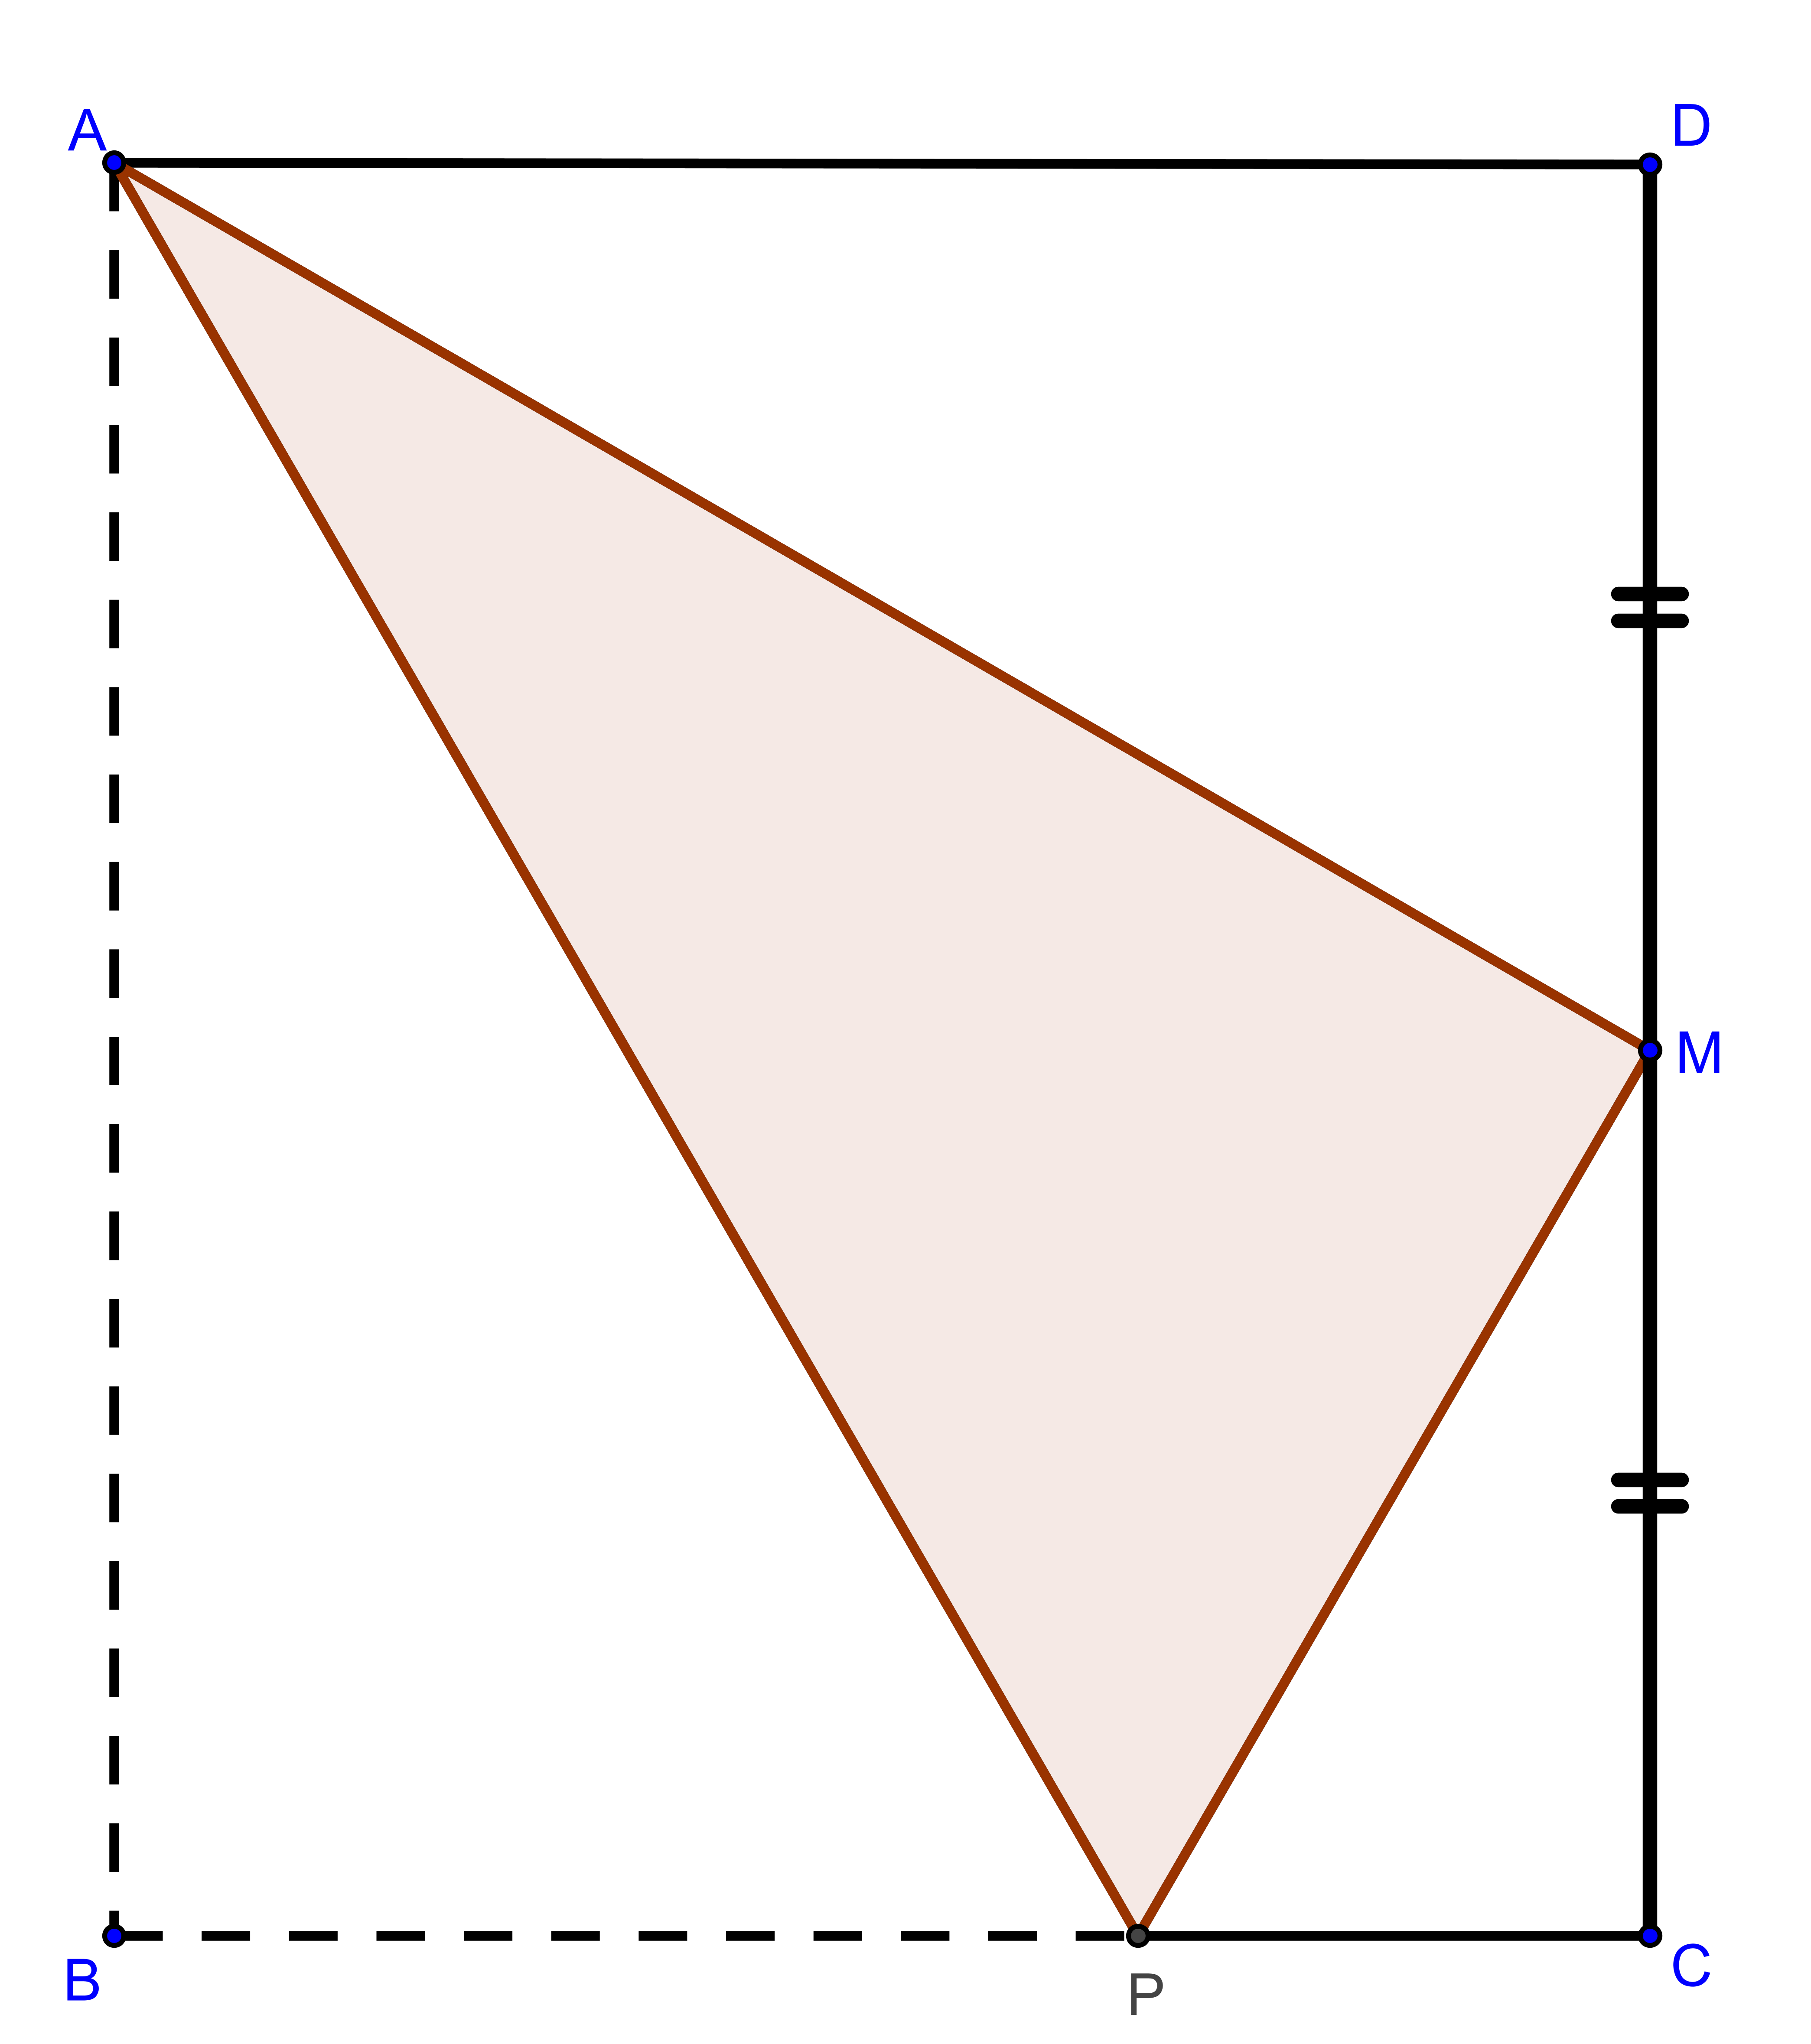
\includegraphics[width=0.35\textwidth]{top_math_p76_03}
\ep

\bp
\(AB=10\), \(AC=12\), \(BC=15\), \(\triangle ABC=48\)이고 \(\square PQRS\)가 정사각형일 때, \(QC\)의 길이를 구하여라.
\par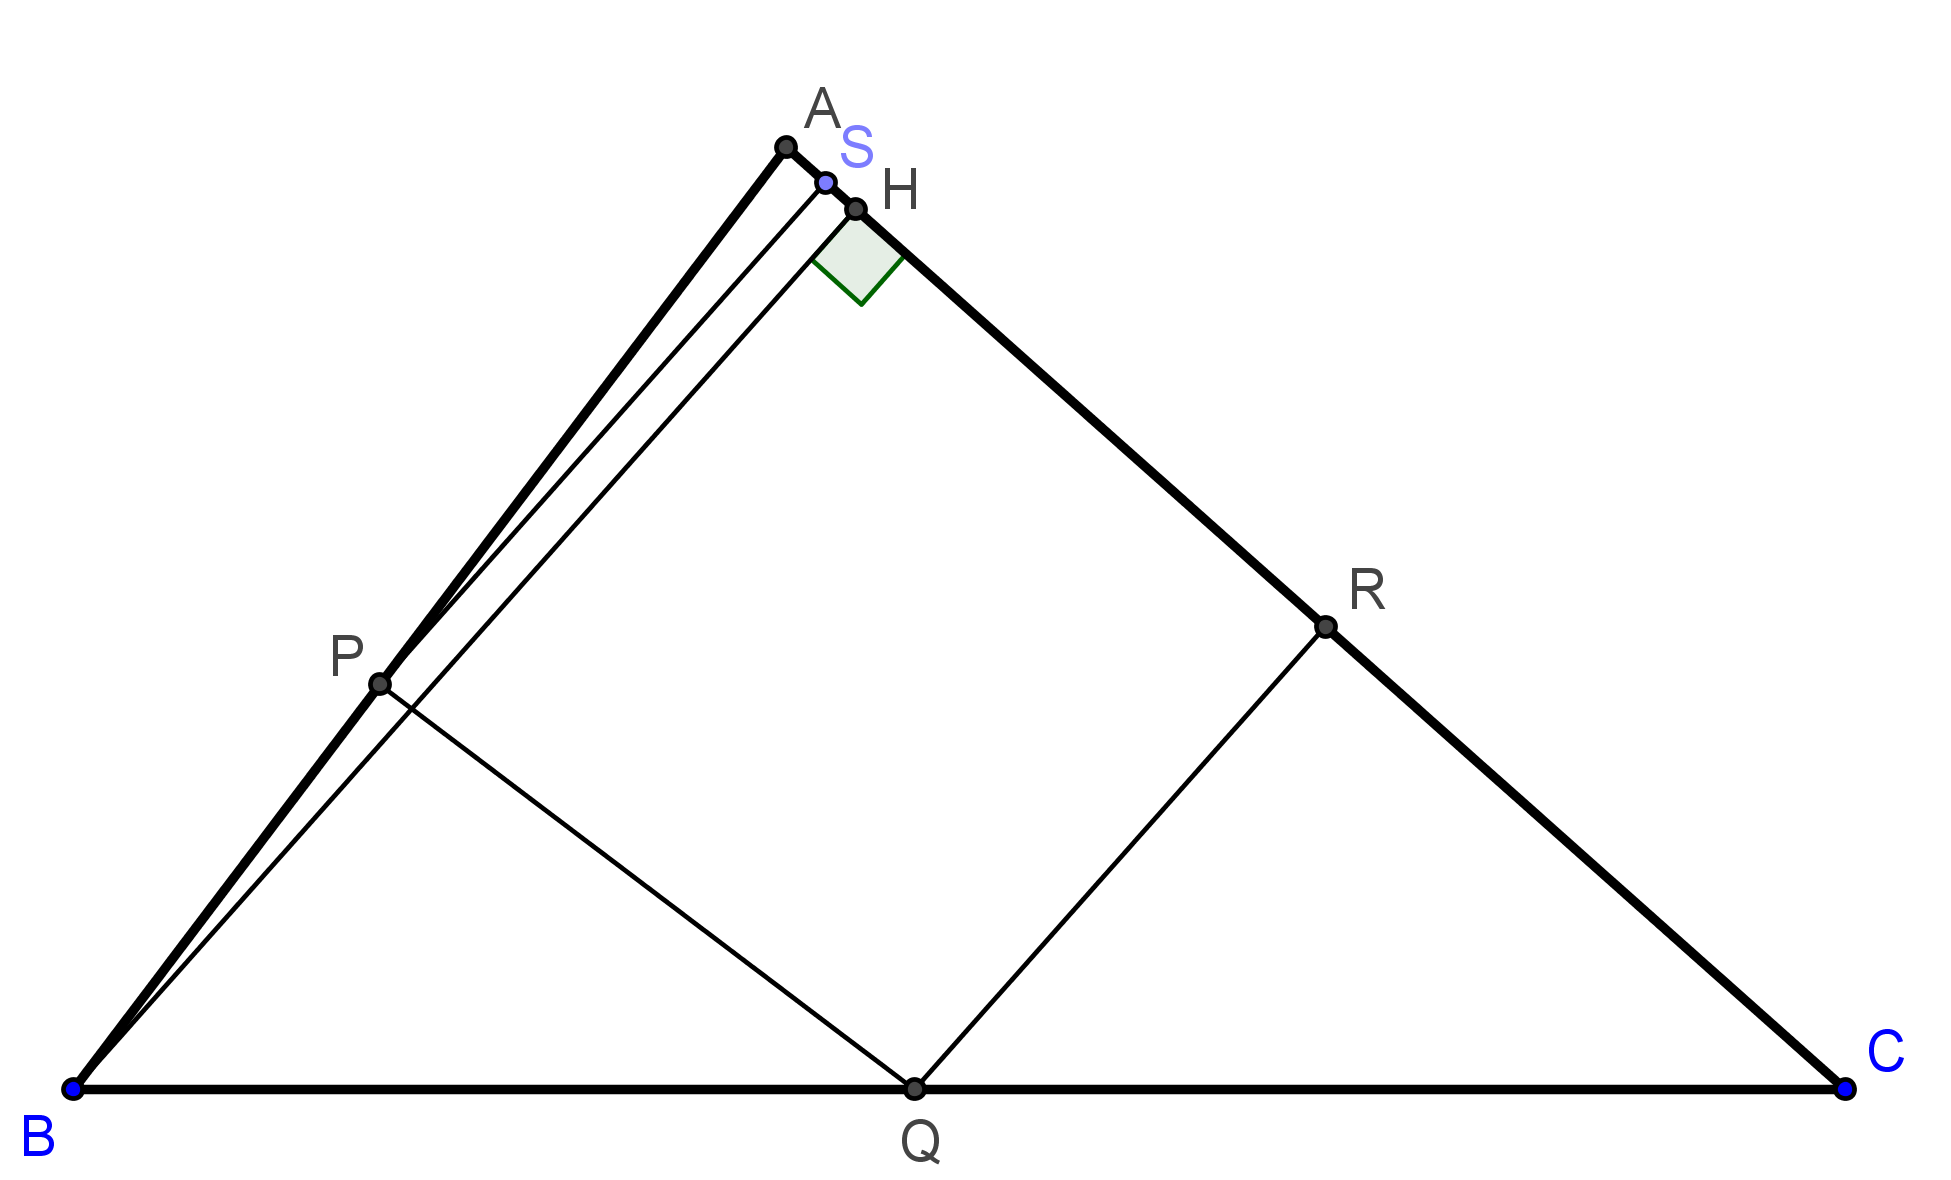
\includegraphics[width=0.5\textwidth]{top_math_p80_02}
\ep

\bp
\(AD=1\), \(BC=3\), \(DP:PC=1:2\)일 때, \(\triangle ABP:(\triangle PDA+\triangle PBC)\)를 구하여라.
\par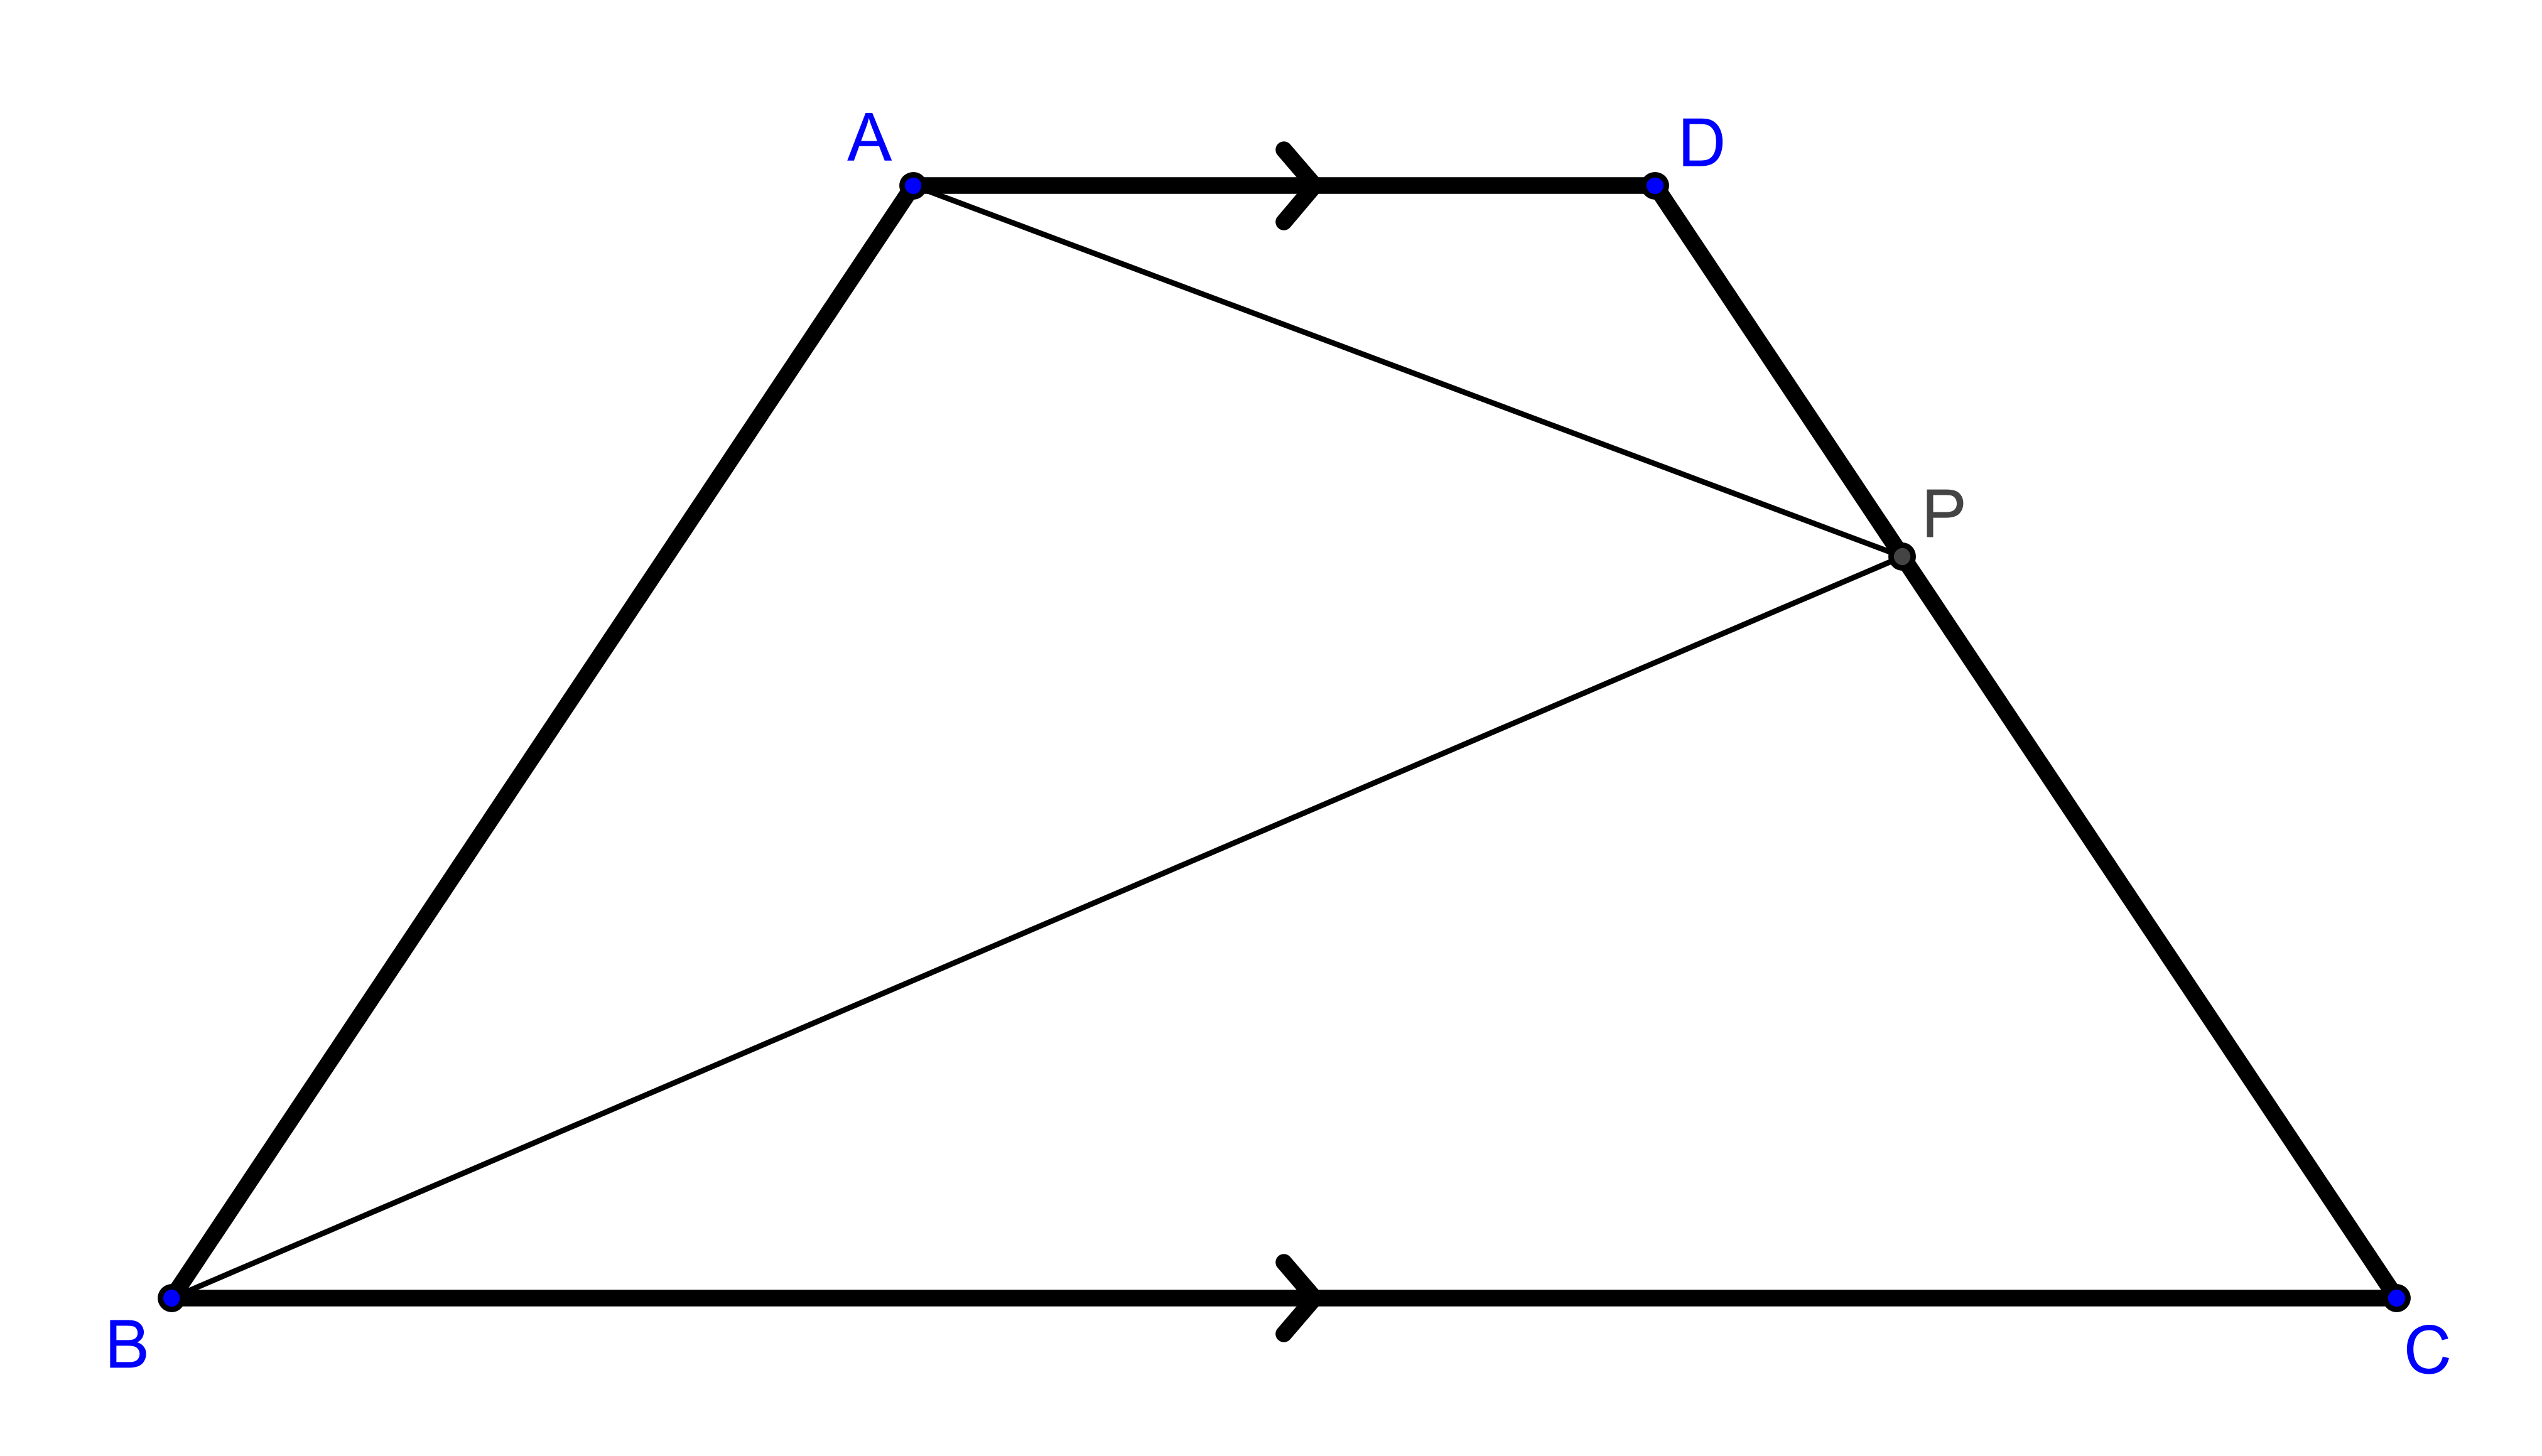
\includegraphics[width=0.5\textwidth]{top_math_p80_04}
\ep

\bp
\(AB=8\), \(BC=7\), \(CA=6\), \(\angle PAC=\angle PBA\)일 때, \(PC\)의 길이를 구하여라.
\par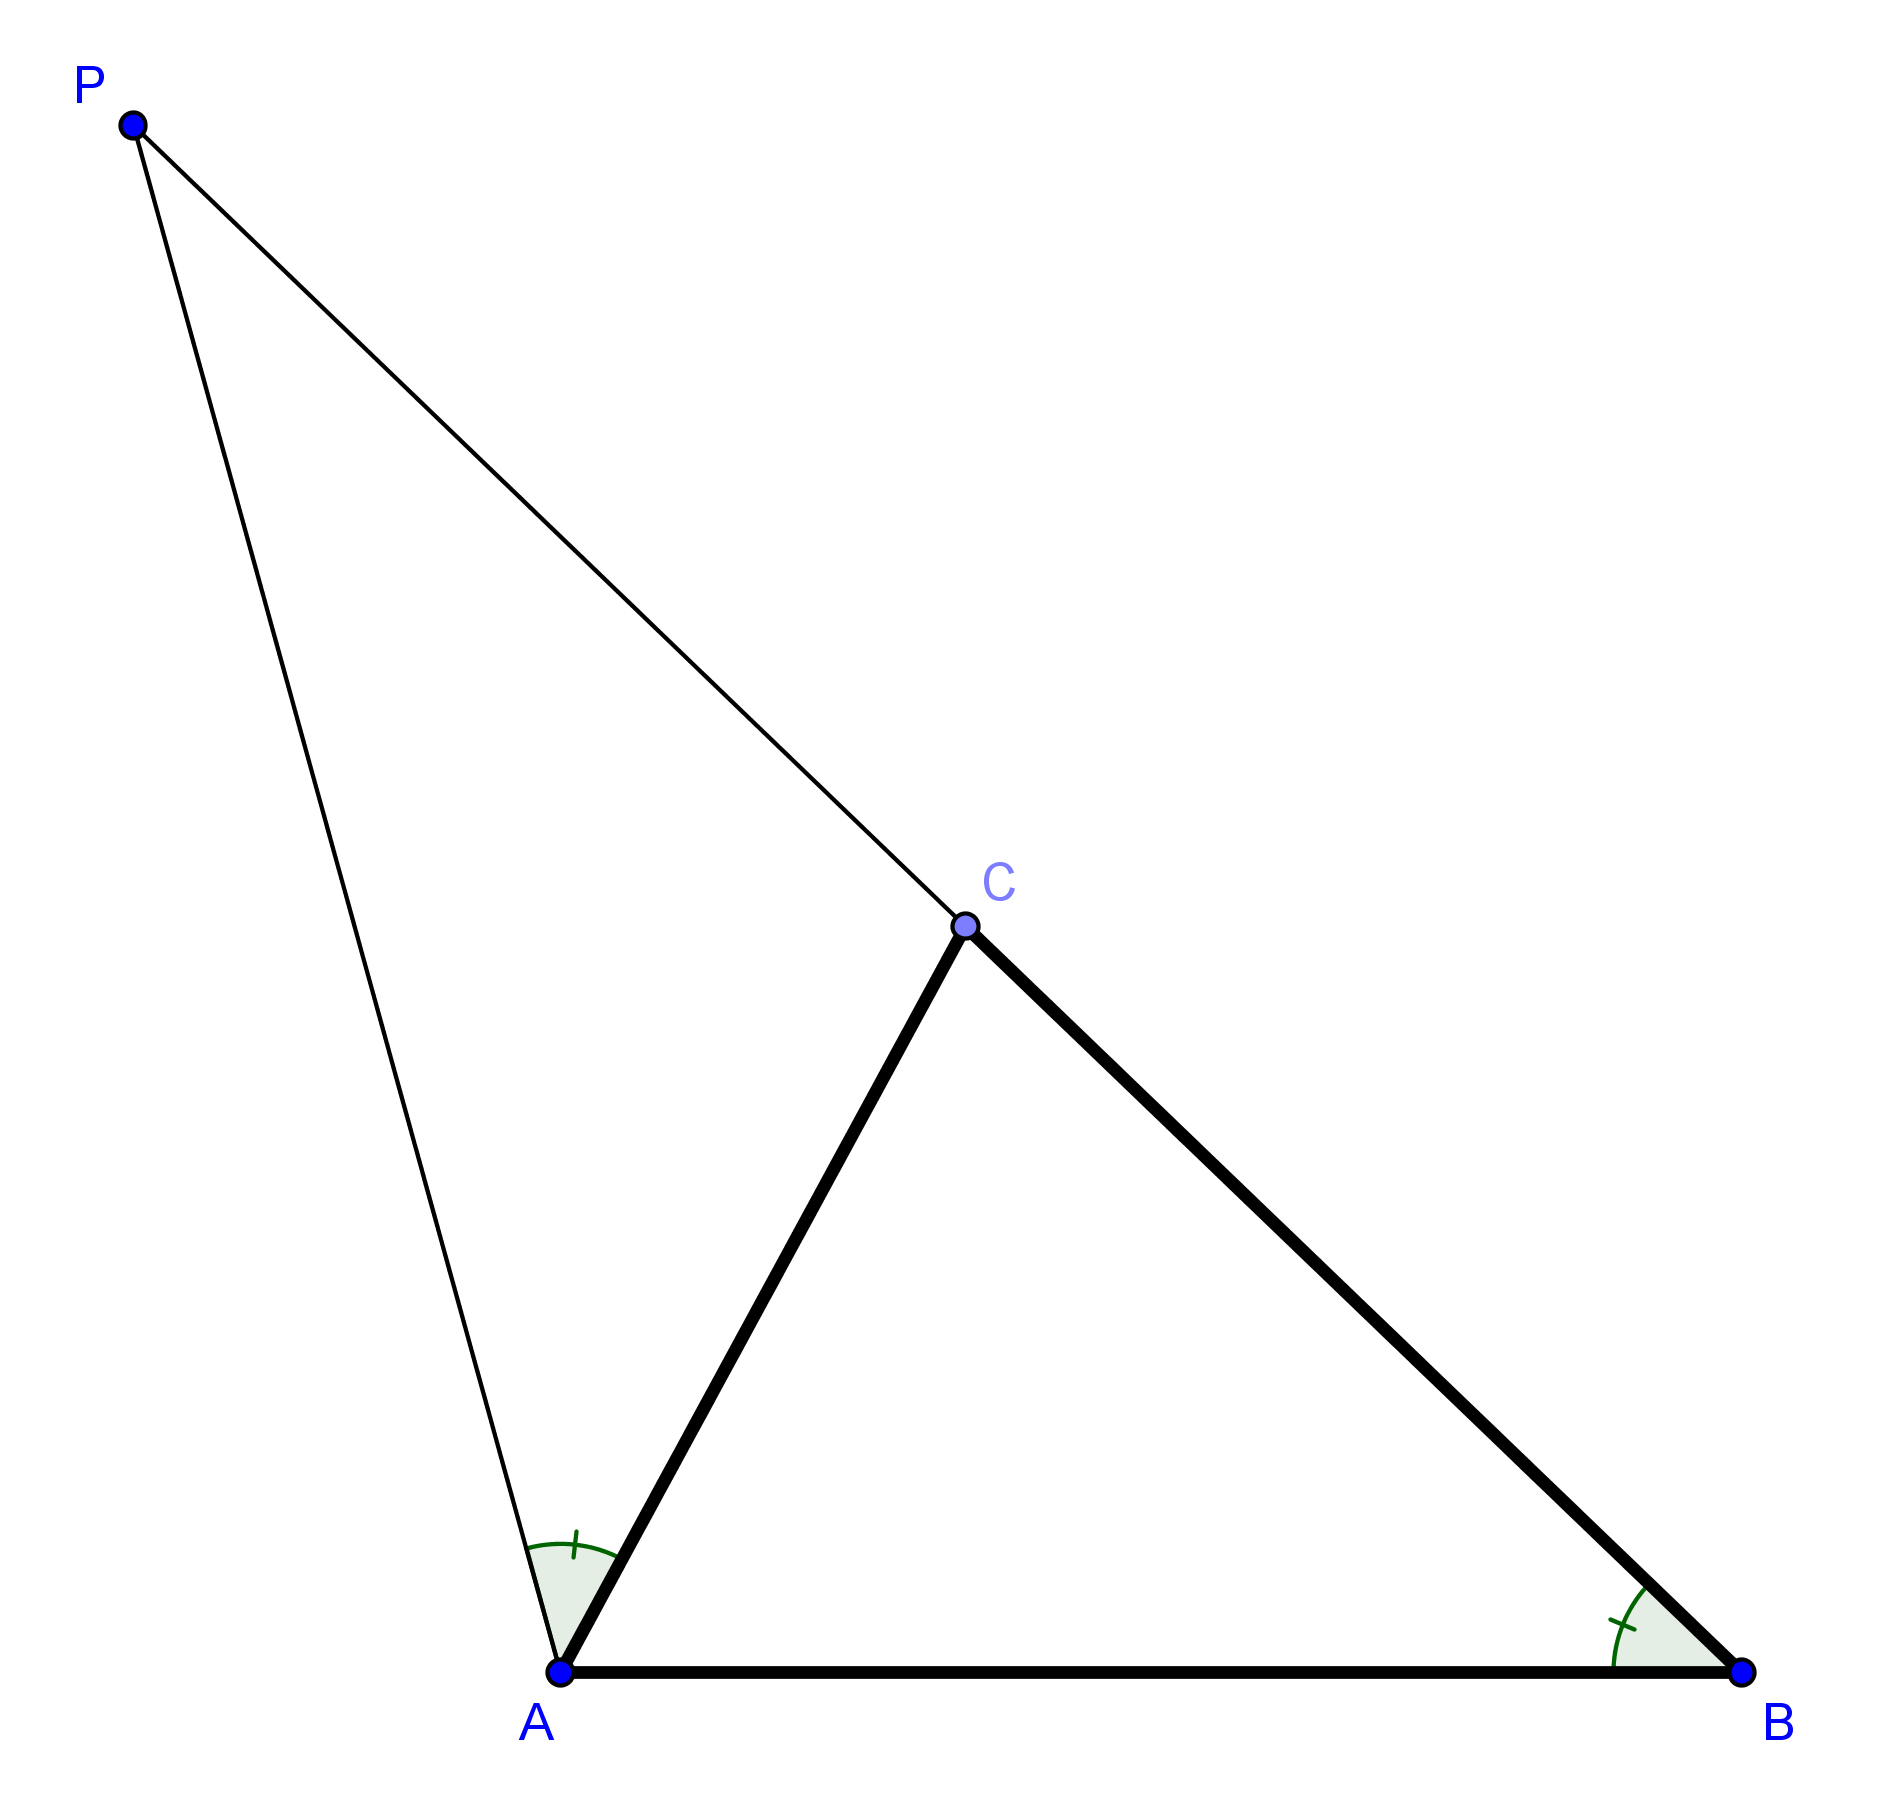
\includegraphics[width=0.5\textwidth]{top_math_p80_05}
\ep

\bp
\(\triangle ABE\), \(\triangle BCF\), \(\triangle CDG\)는 모두 정삼각형이고, \(E\), \(F\), \(G\), \(H\)는 한 직선 위에 있다.
\(AE=4\), \(AH=12\)일 때, \(CG\)의 길이를 구하여라.
\par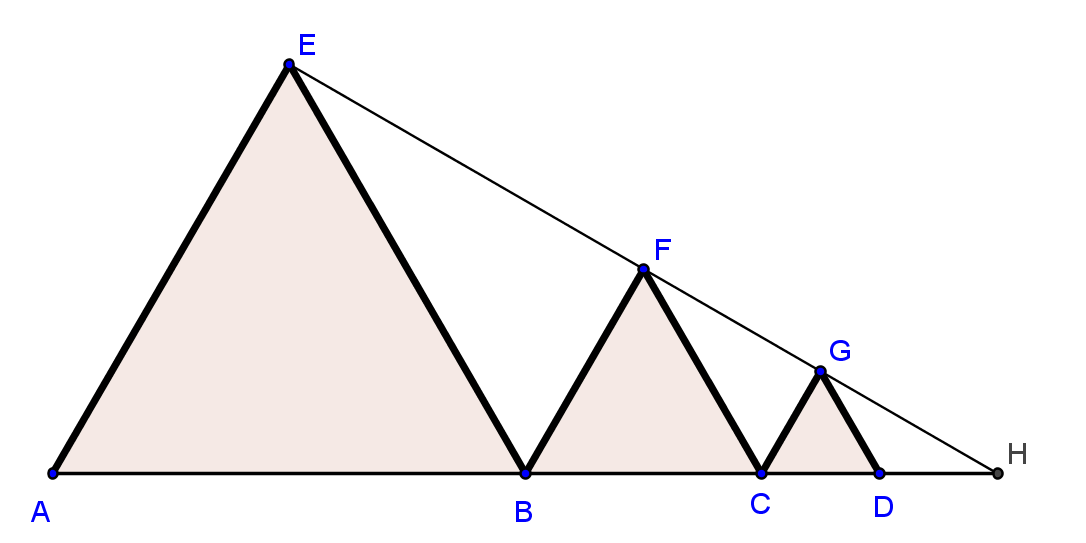
\includegraphics[width=0.5\textwidth]{top_math_p81_07}
\ep

\bp
\(\angle ADE\)의 크기를 구하여라(\(BC=BE\)).
\par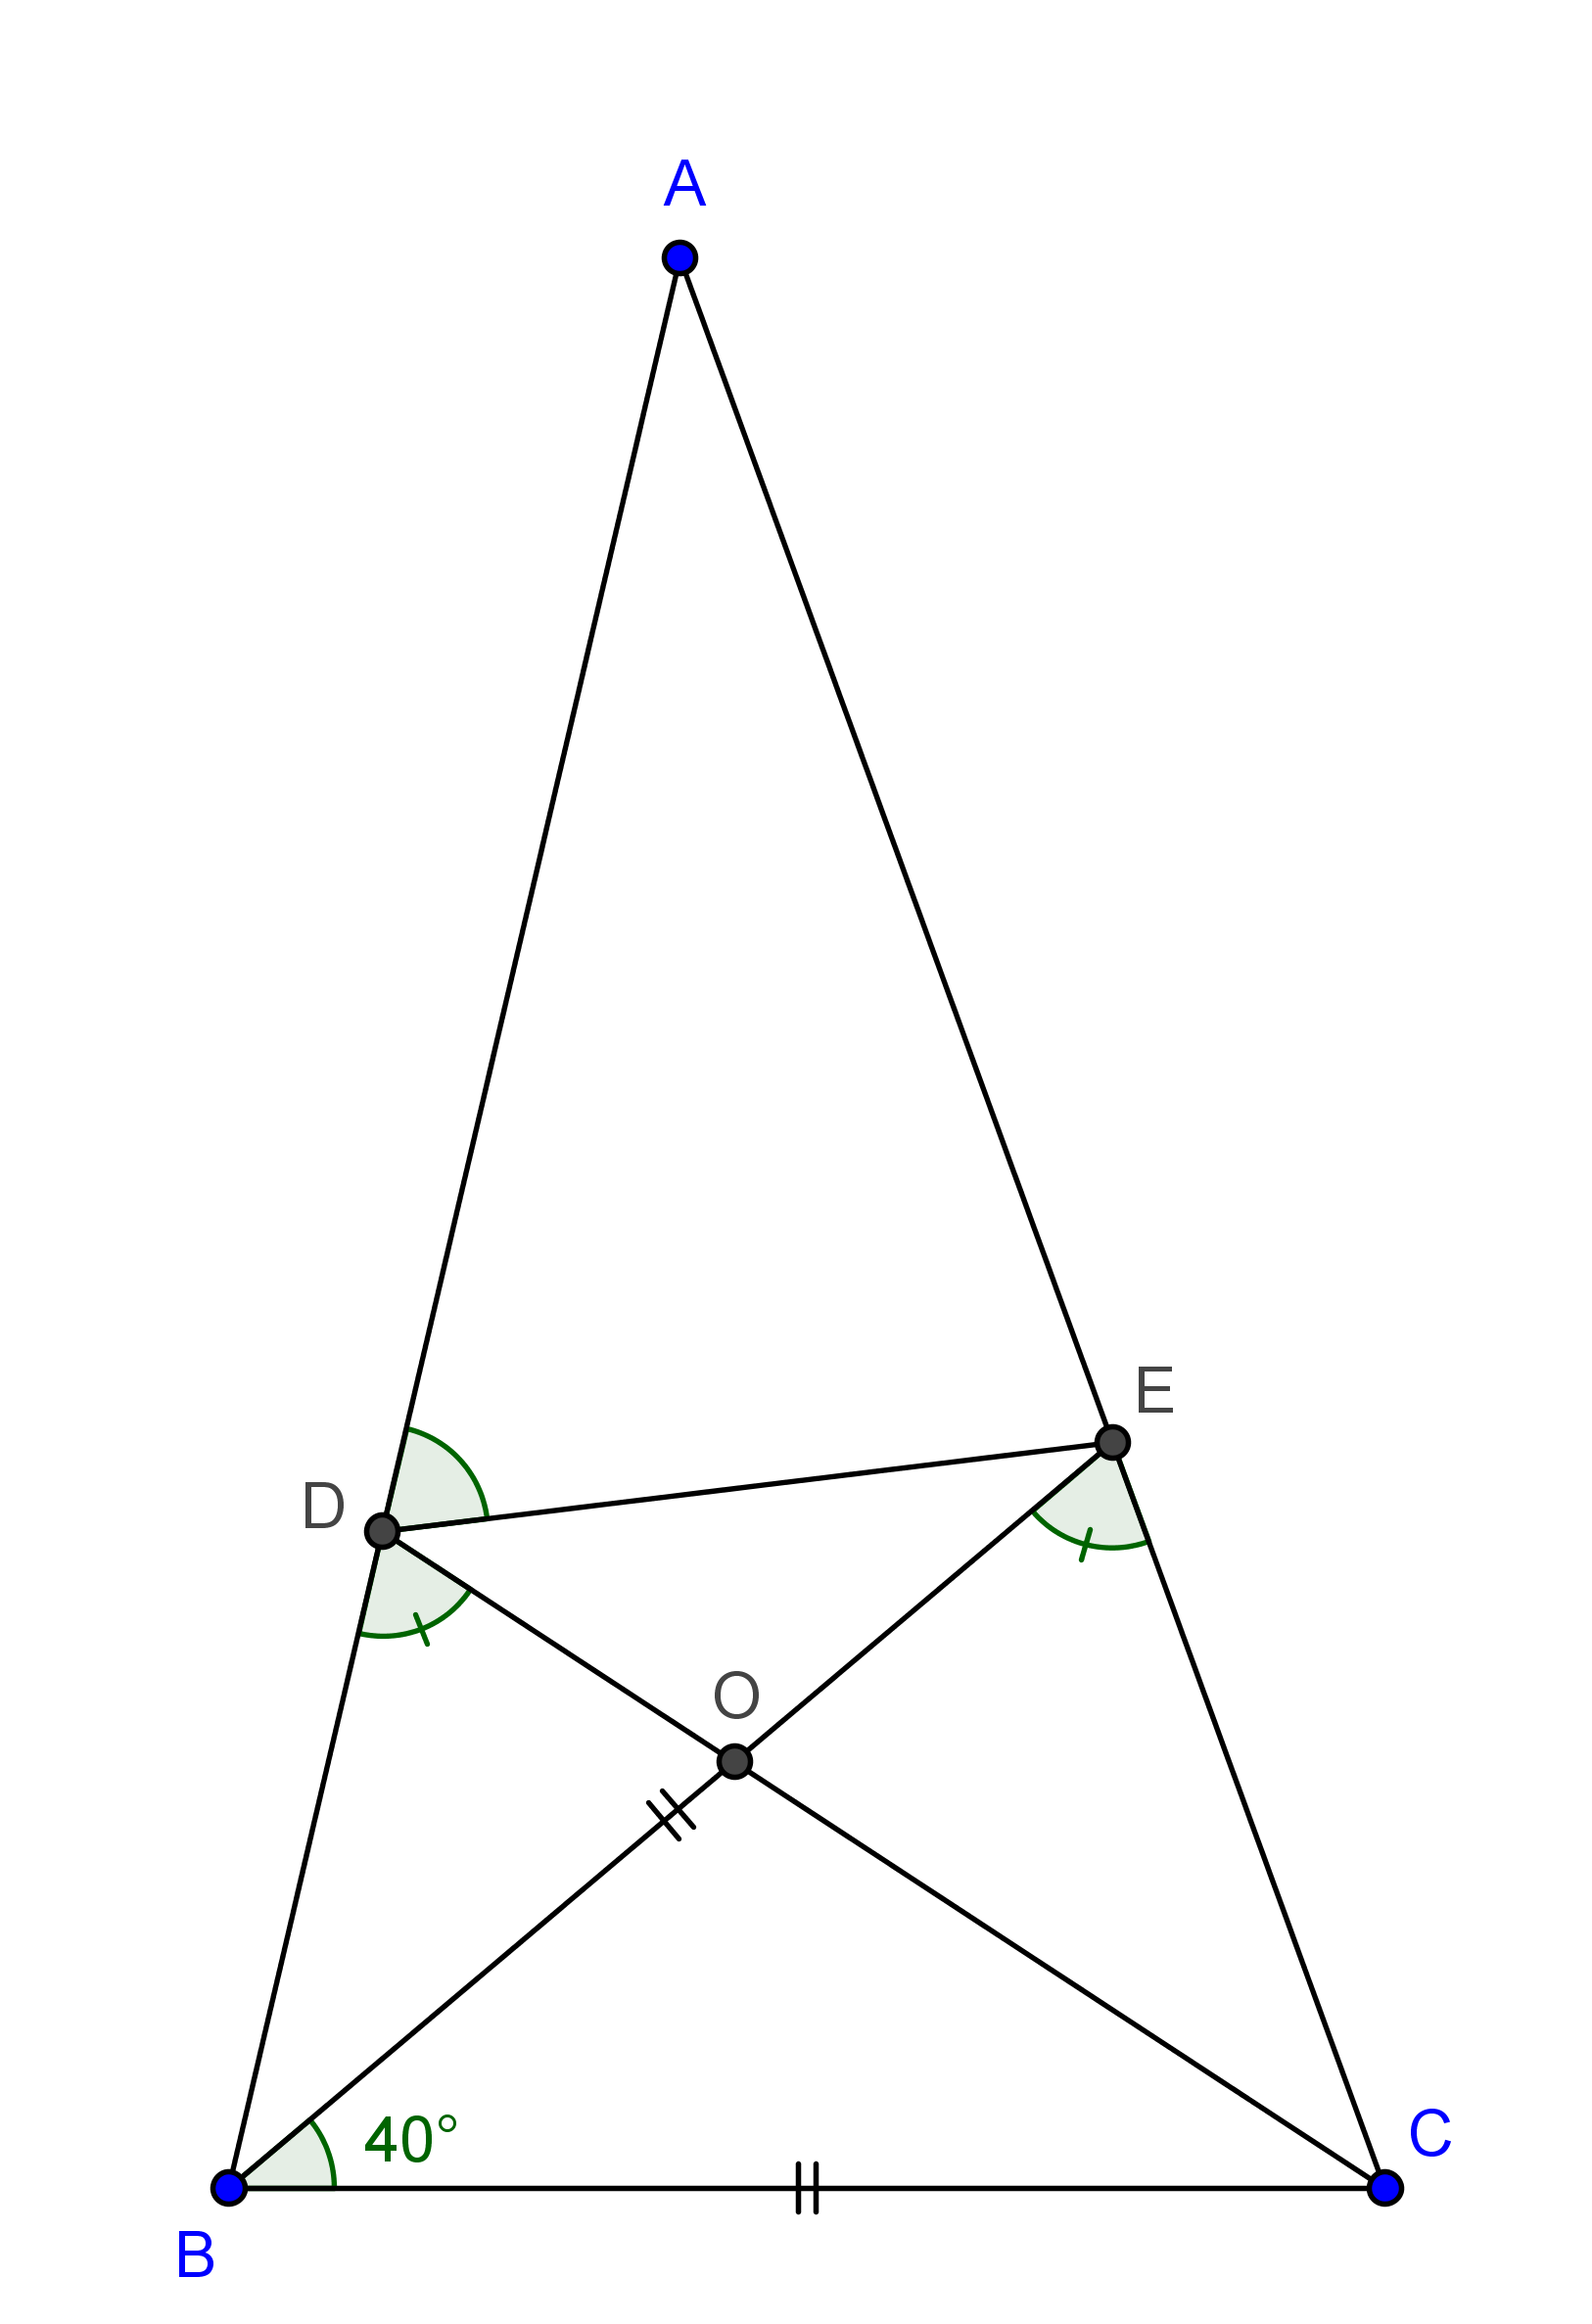
\includegraphics[width=0.3\textwidth]{top_math_p81_08}
\ep

\bp
등변사다리꼴 \(ABCD\)에서 \(AC=BD=BC=3AB\)이고, \(AB\parall DE\)일 때, \(BE:EC\)를 구하여라.
\par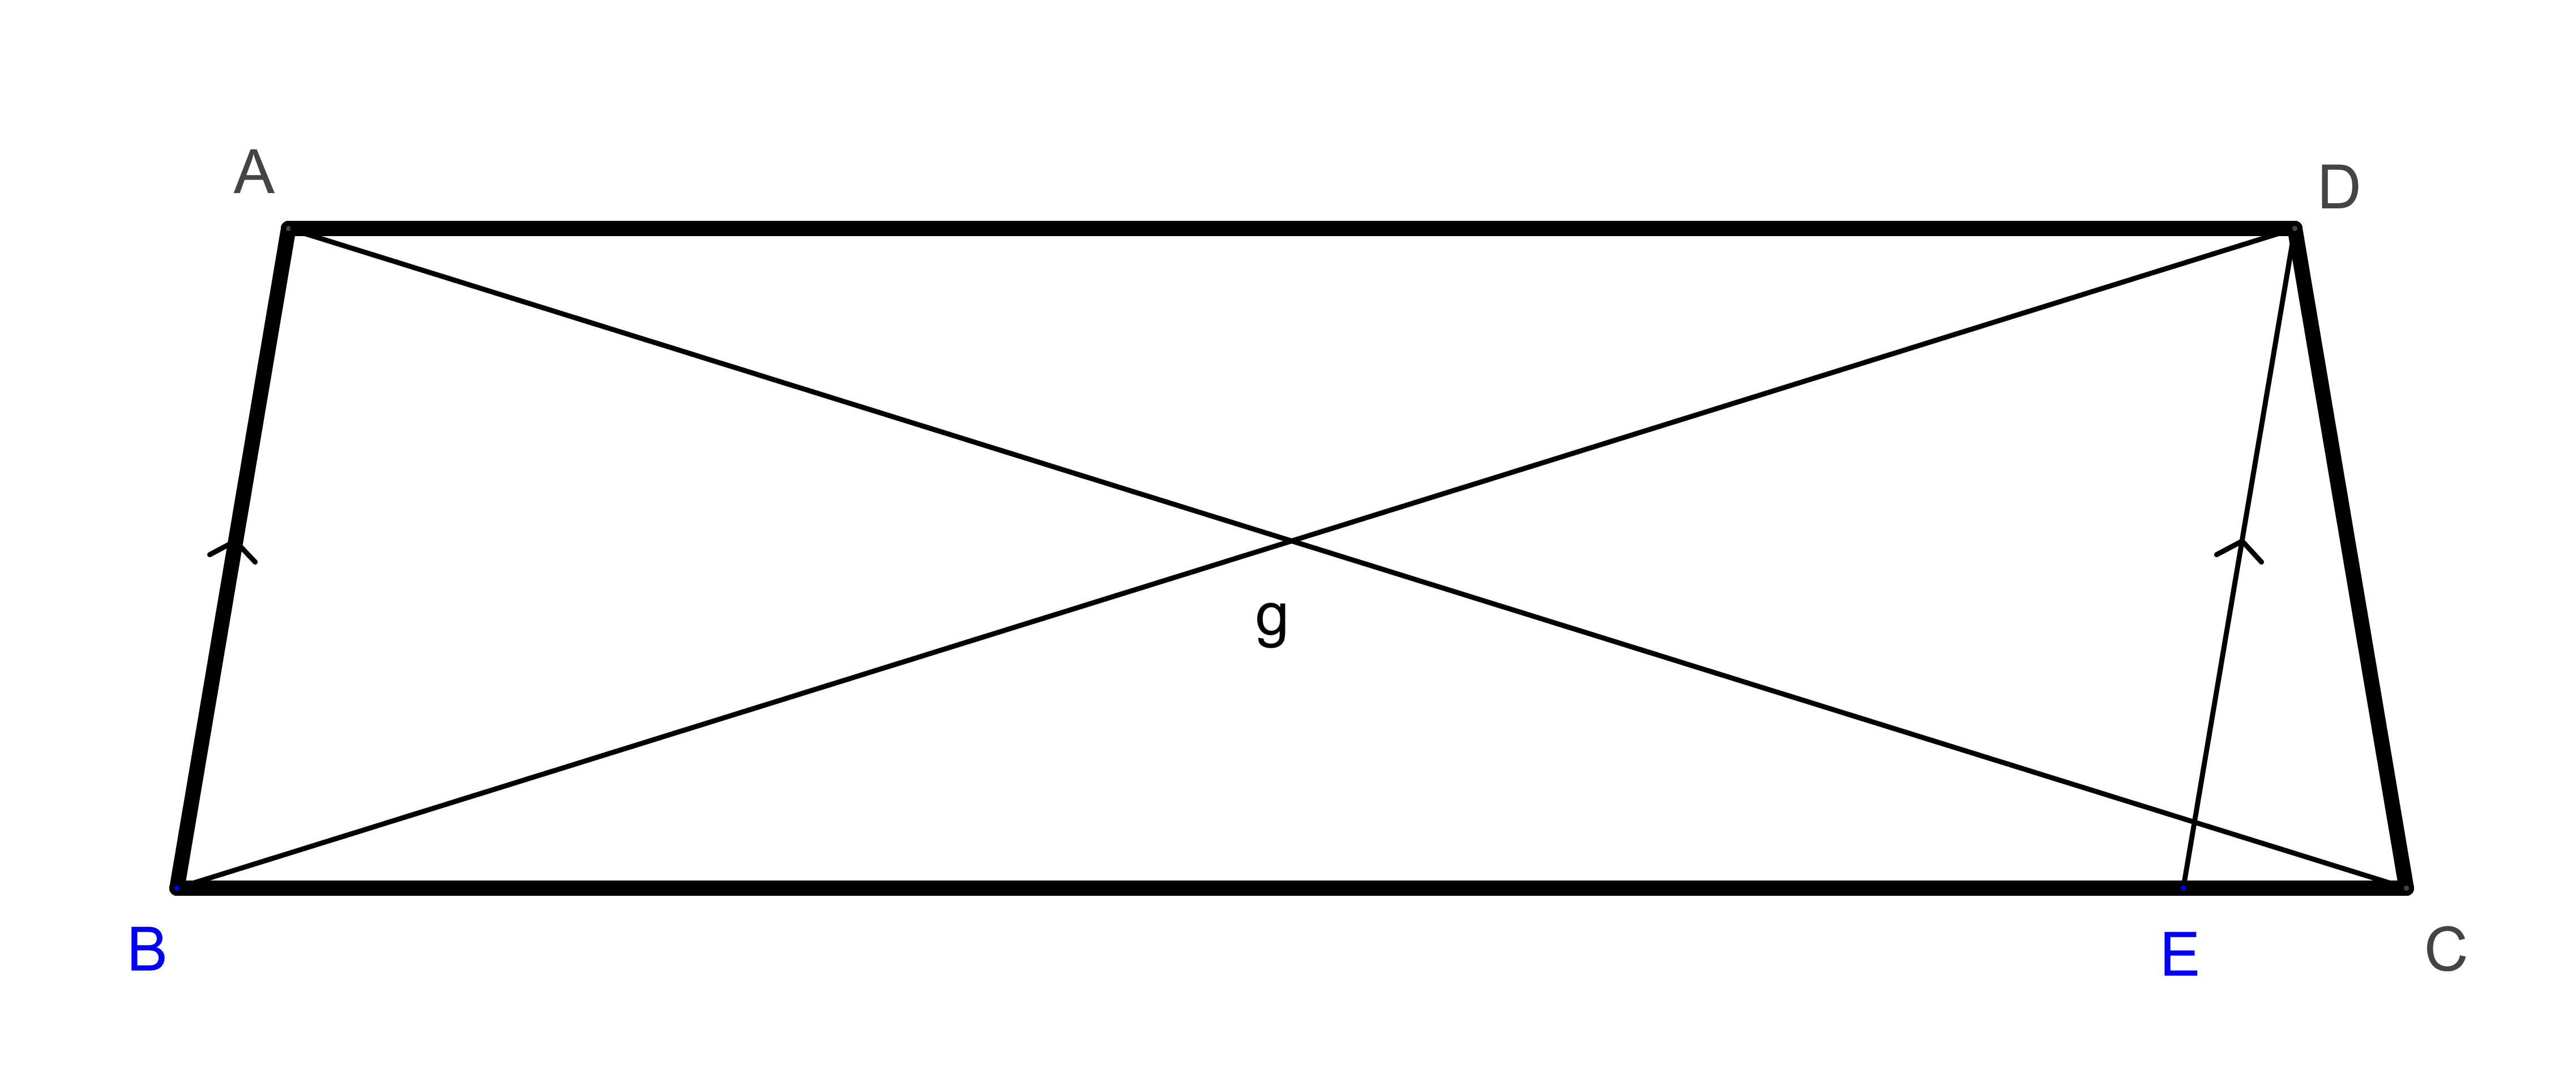
\includegraphics[width=0.5\textwidth]{top_math_p81_09}
\ep

\bp
직각삼각형 \(ABC\)에 정사각형 \(DEFG\)가 내접한다.
\(DH=a\), \(HI=b\), \(IG=c\)라고 할 때, \(a\), \(b\), \(c\) 사이의 관계식을 구하여라.
\par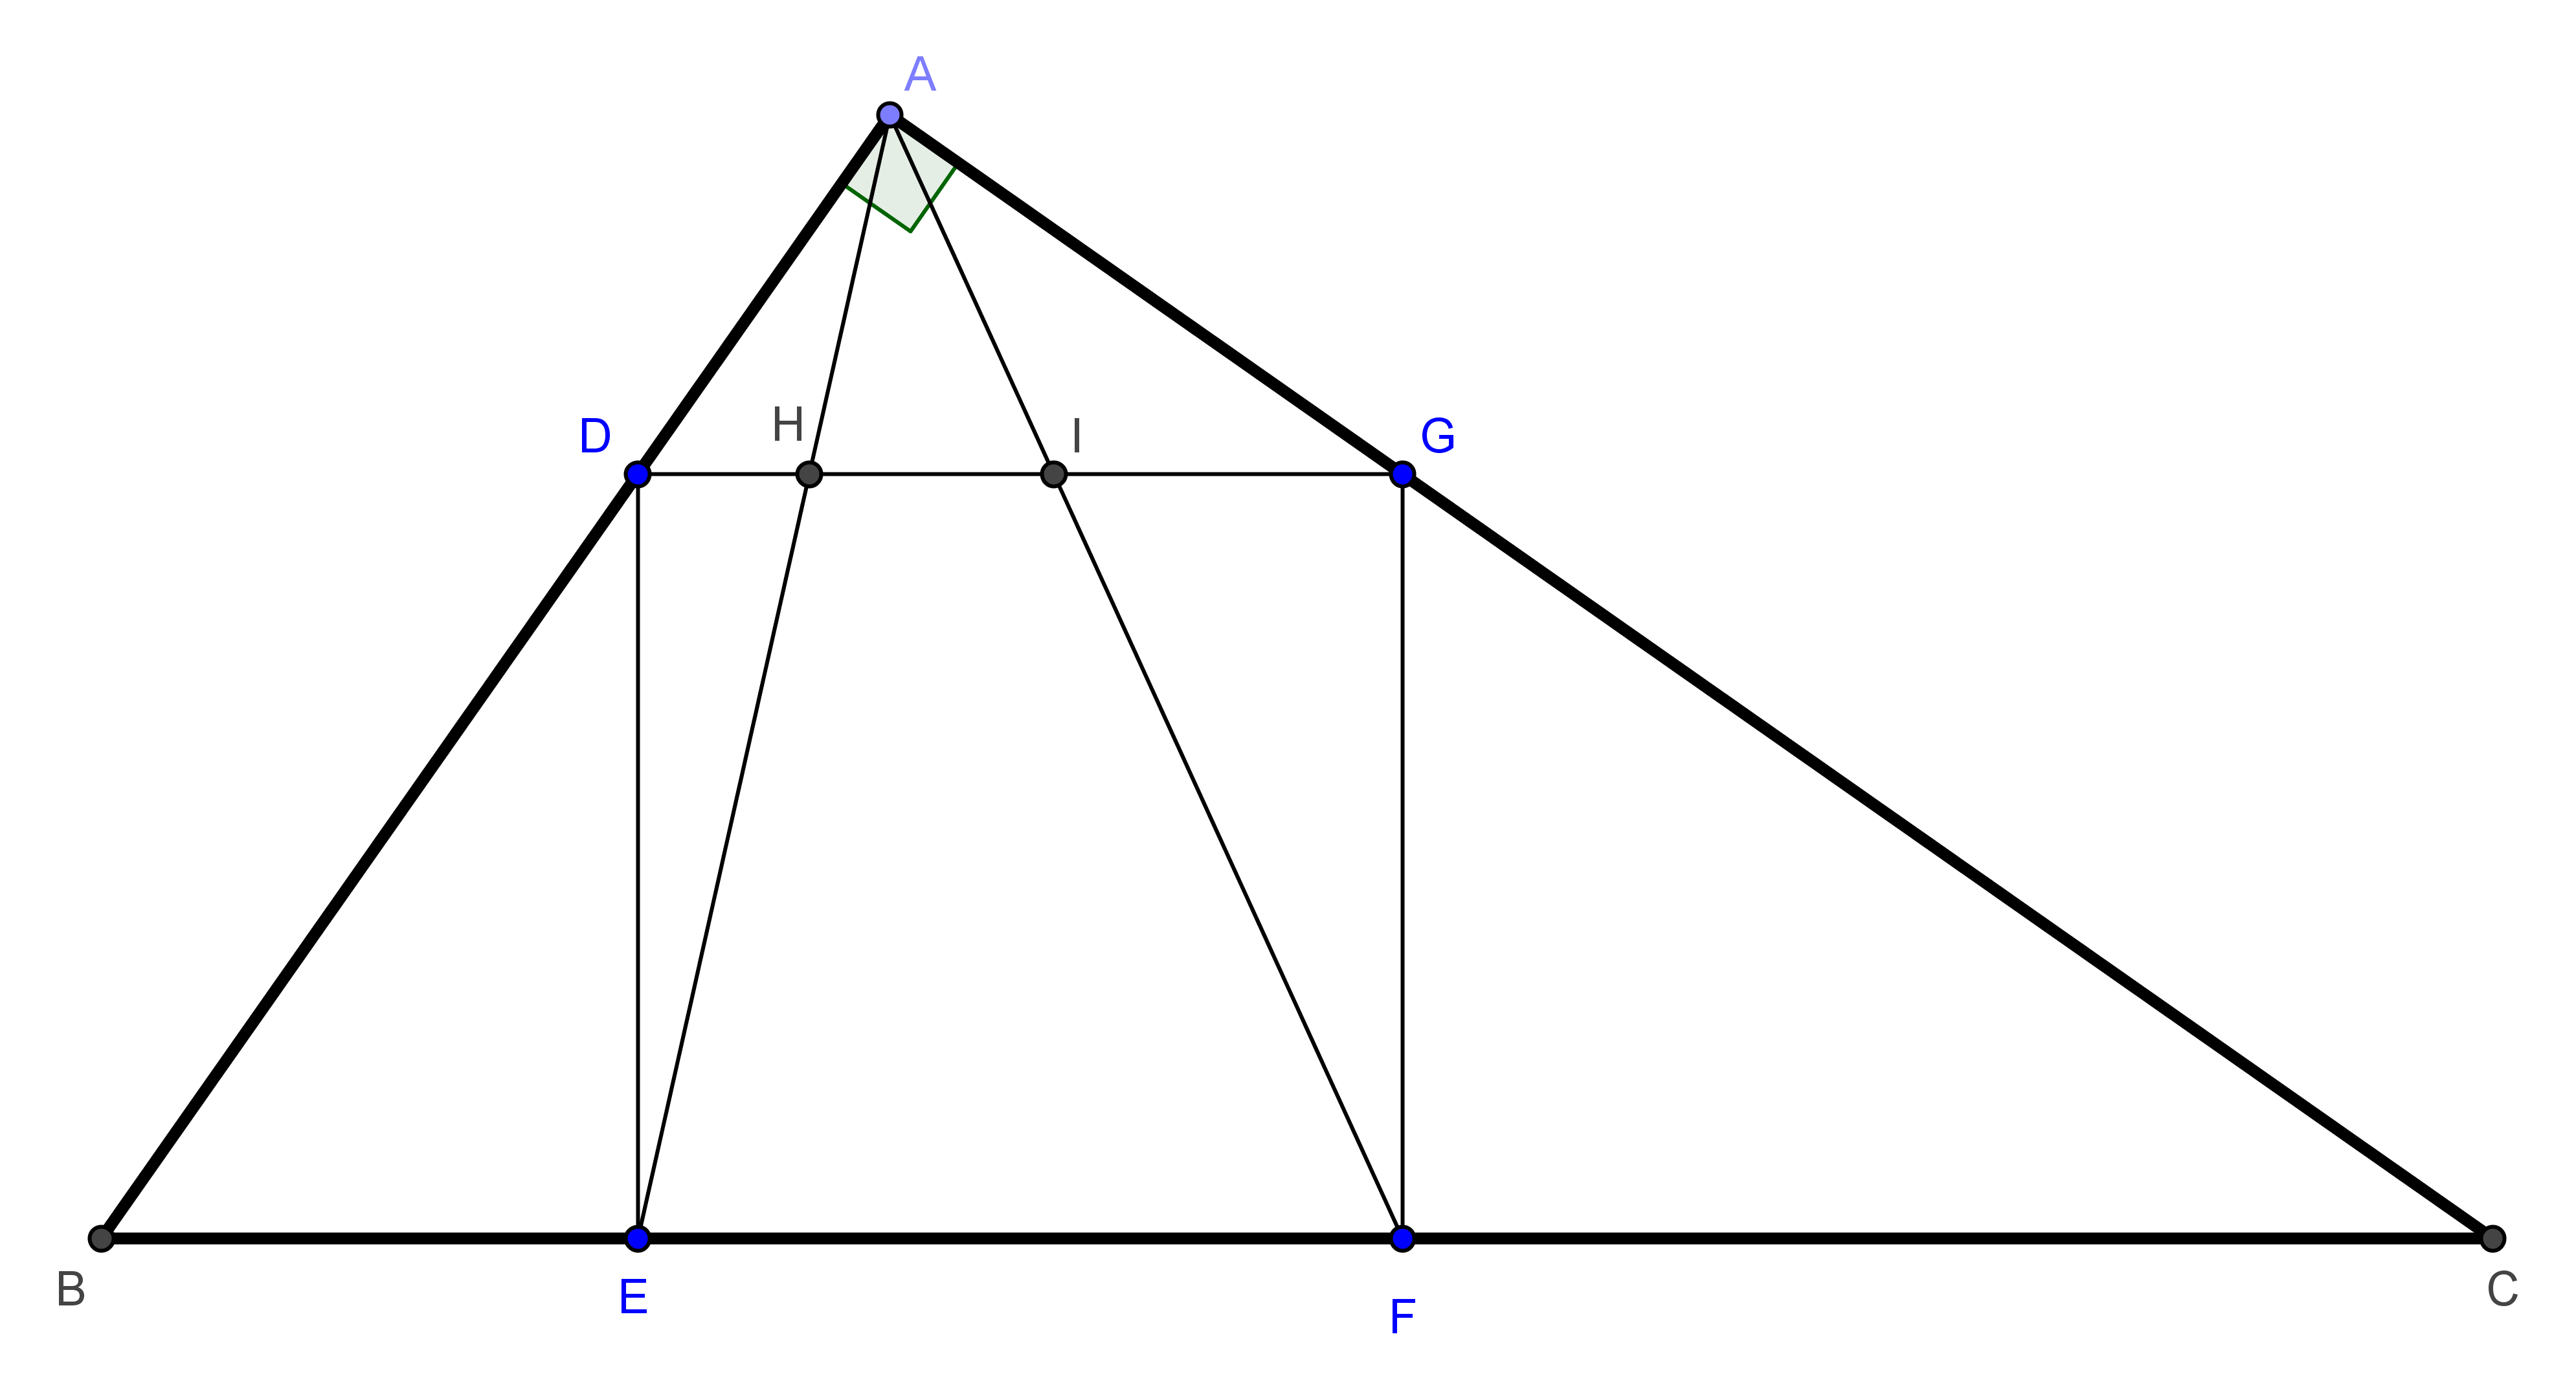
\includegraphics[width=0.65\textwidth]{top_math_p81_10}
\bigskip
\ep

\bp
\(I\)는 \(\triangle ABC\)의 내심이고, \(AB=5\), \(BC=6\), \(CA=7\)일 때, \(AI:ID\)를 구하여라.
\par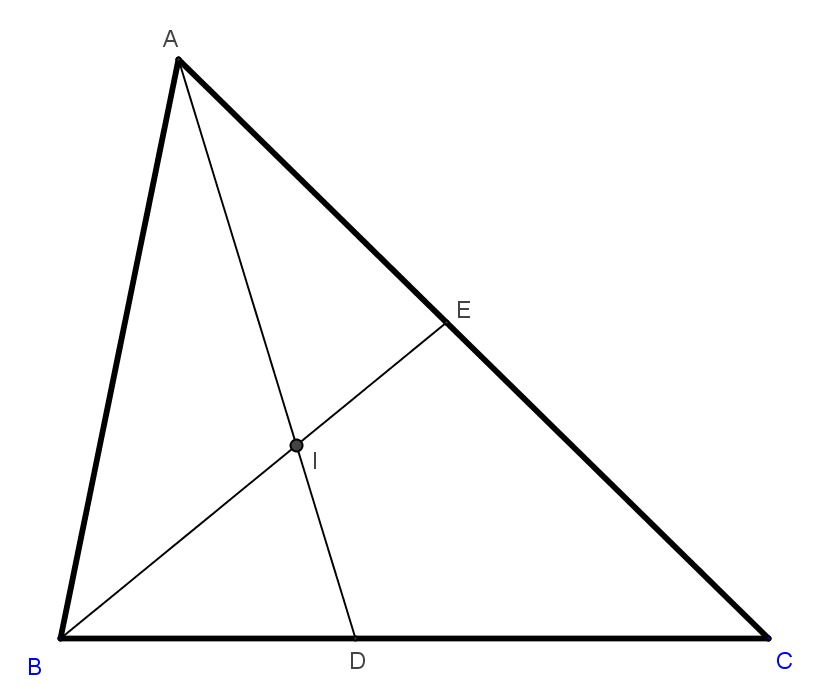
\includegraphics[width=0.5\textwidth]{top_math_p95_07}
\ep

\bp
\(I\)는 \(\triangle ABC\)의 내심이고, \(AB=10\), \(BC=12\), \(CA=8\)일 때, \(\triangle IAB:\triangle IAC\)를 구하여라.
\par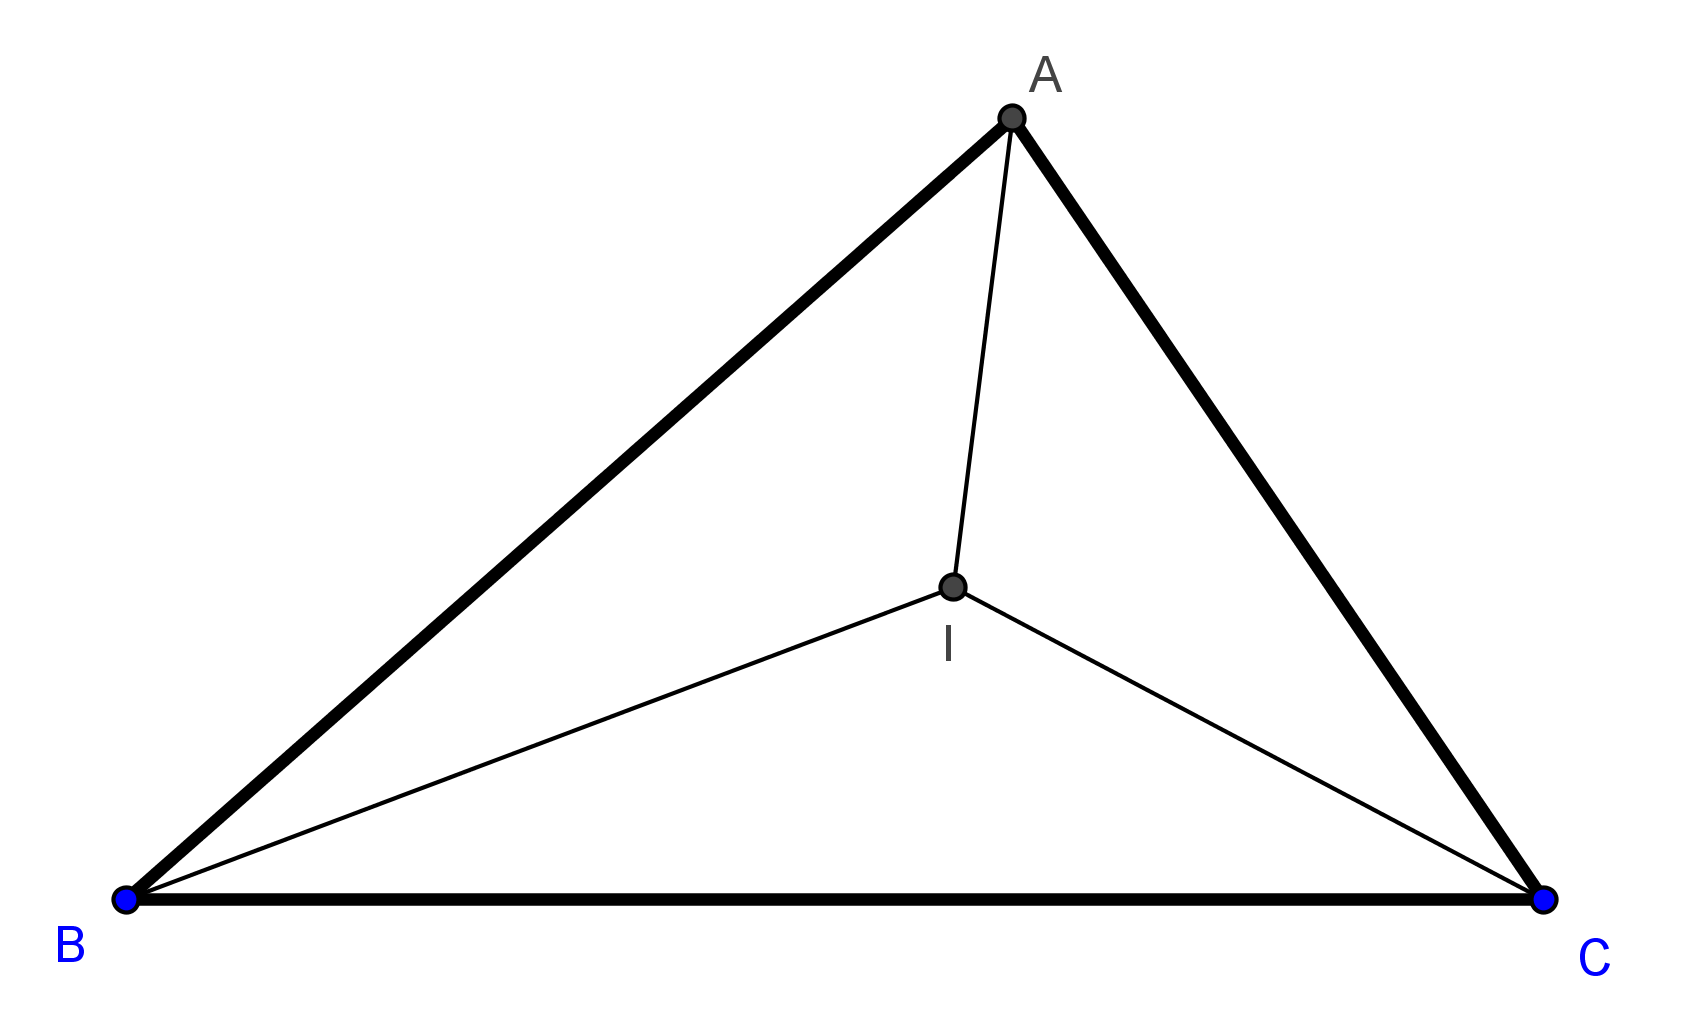
\includegraphics[width=0.5\textwidth]{top_math_p95_08}
\ep

\bp
\(AD=1\), \(BC=3\)일 때, 다음을 구하여라.\\
(1) \(DE:EC\)\\
(2) \(\square ABED:\triangle BCE\)
\par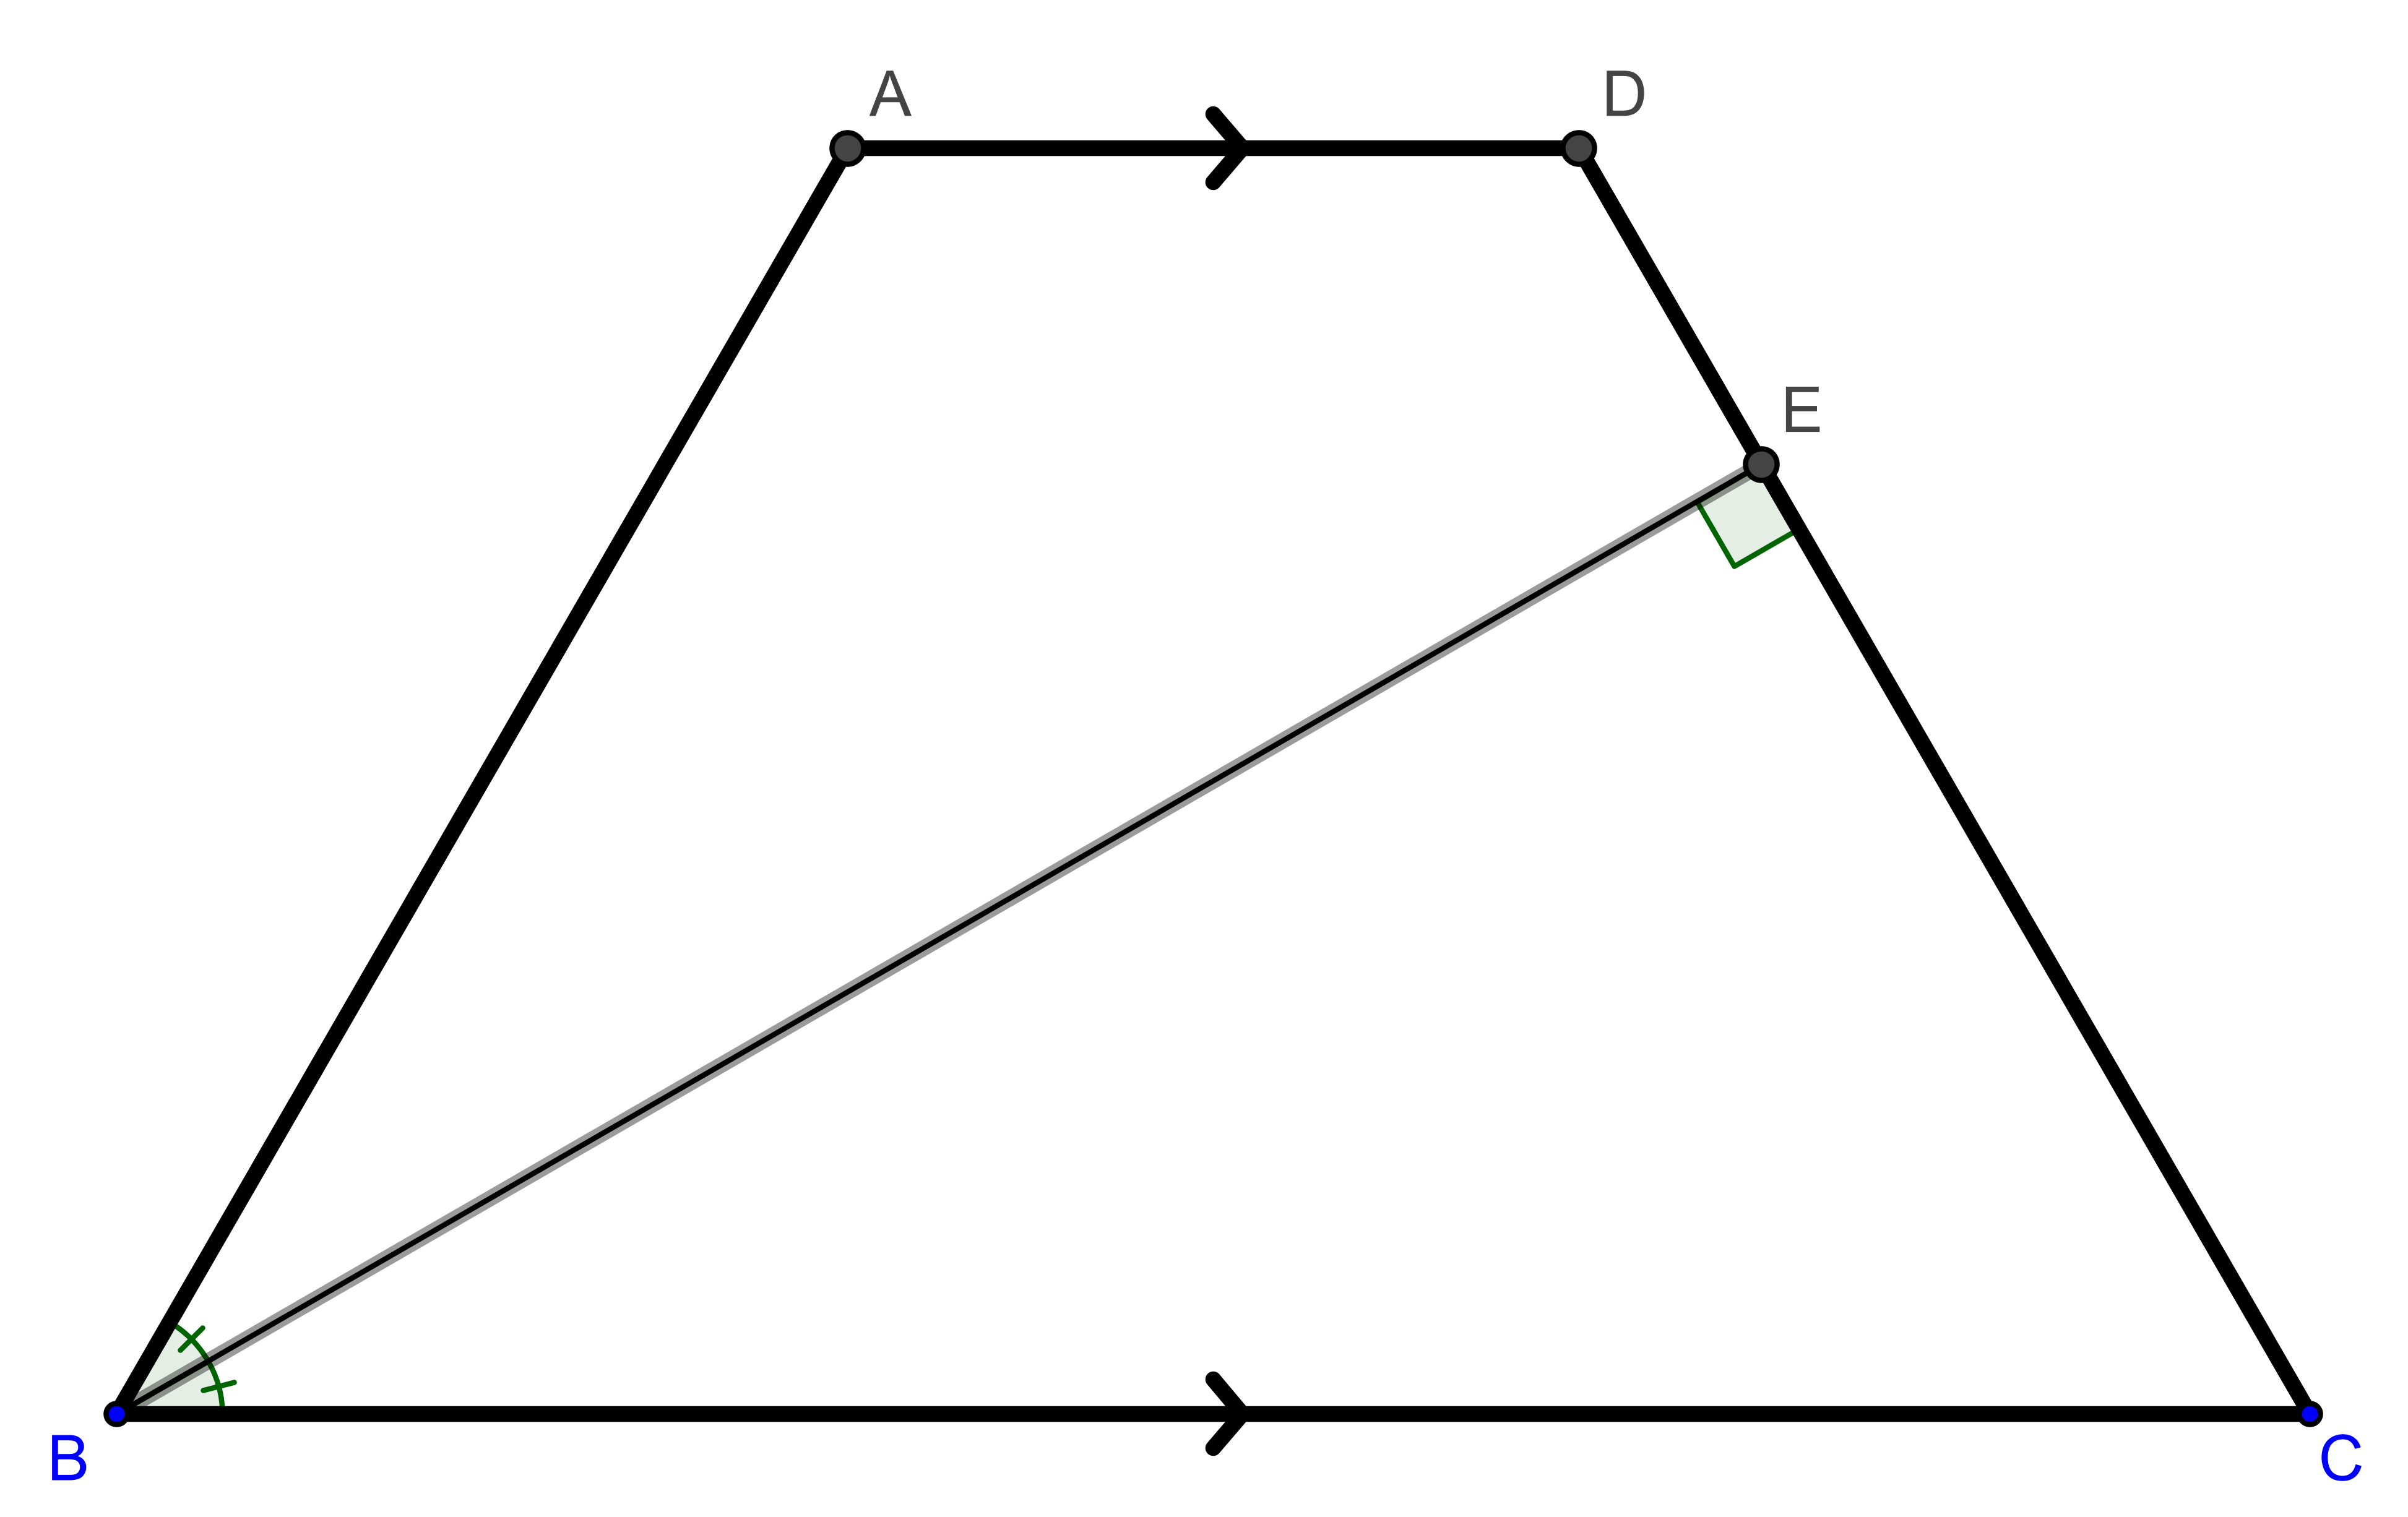
\includegraphics[width=0.5\textwidth]{top_math_p95_10}
\ep

\bp
\(AB=10\), \(CD=10\), \(BC=20\), \(EF=2\)일 때, \(PQ\)의 길이를 구하여라.
\par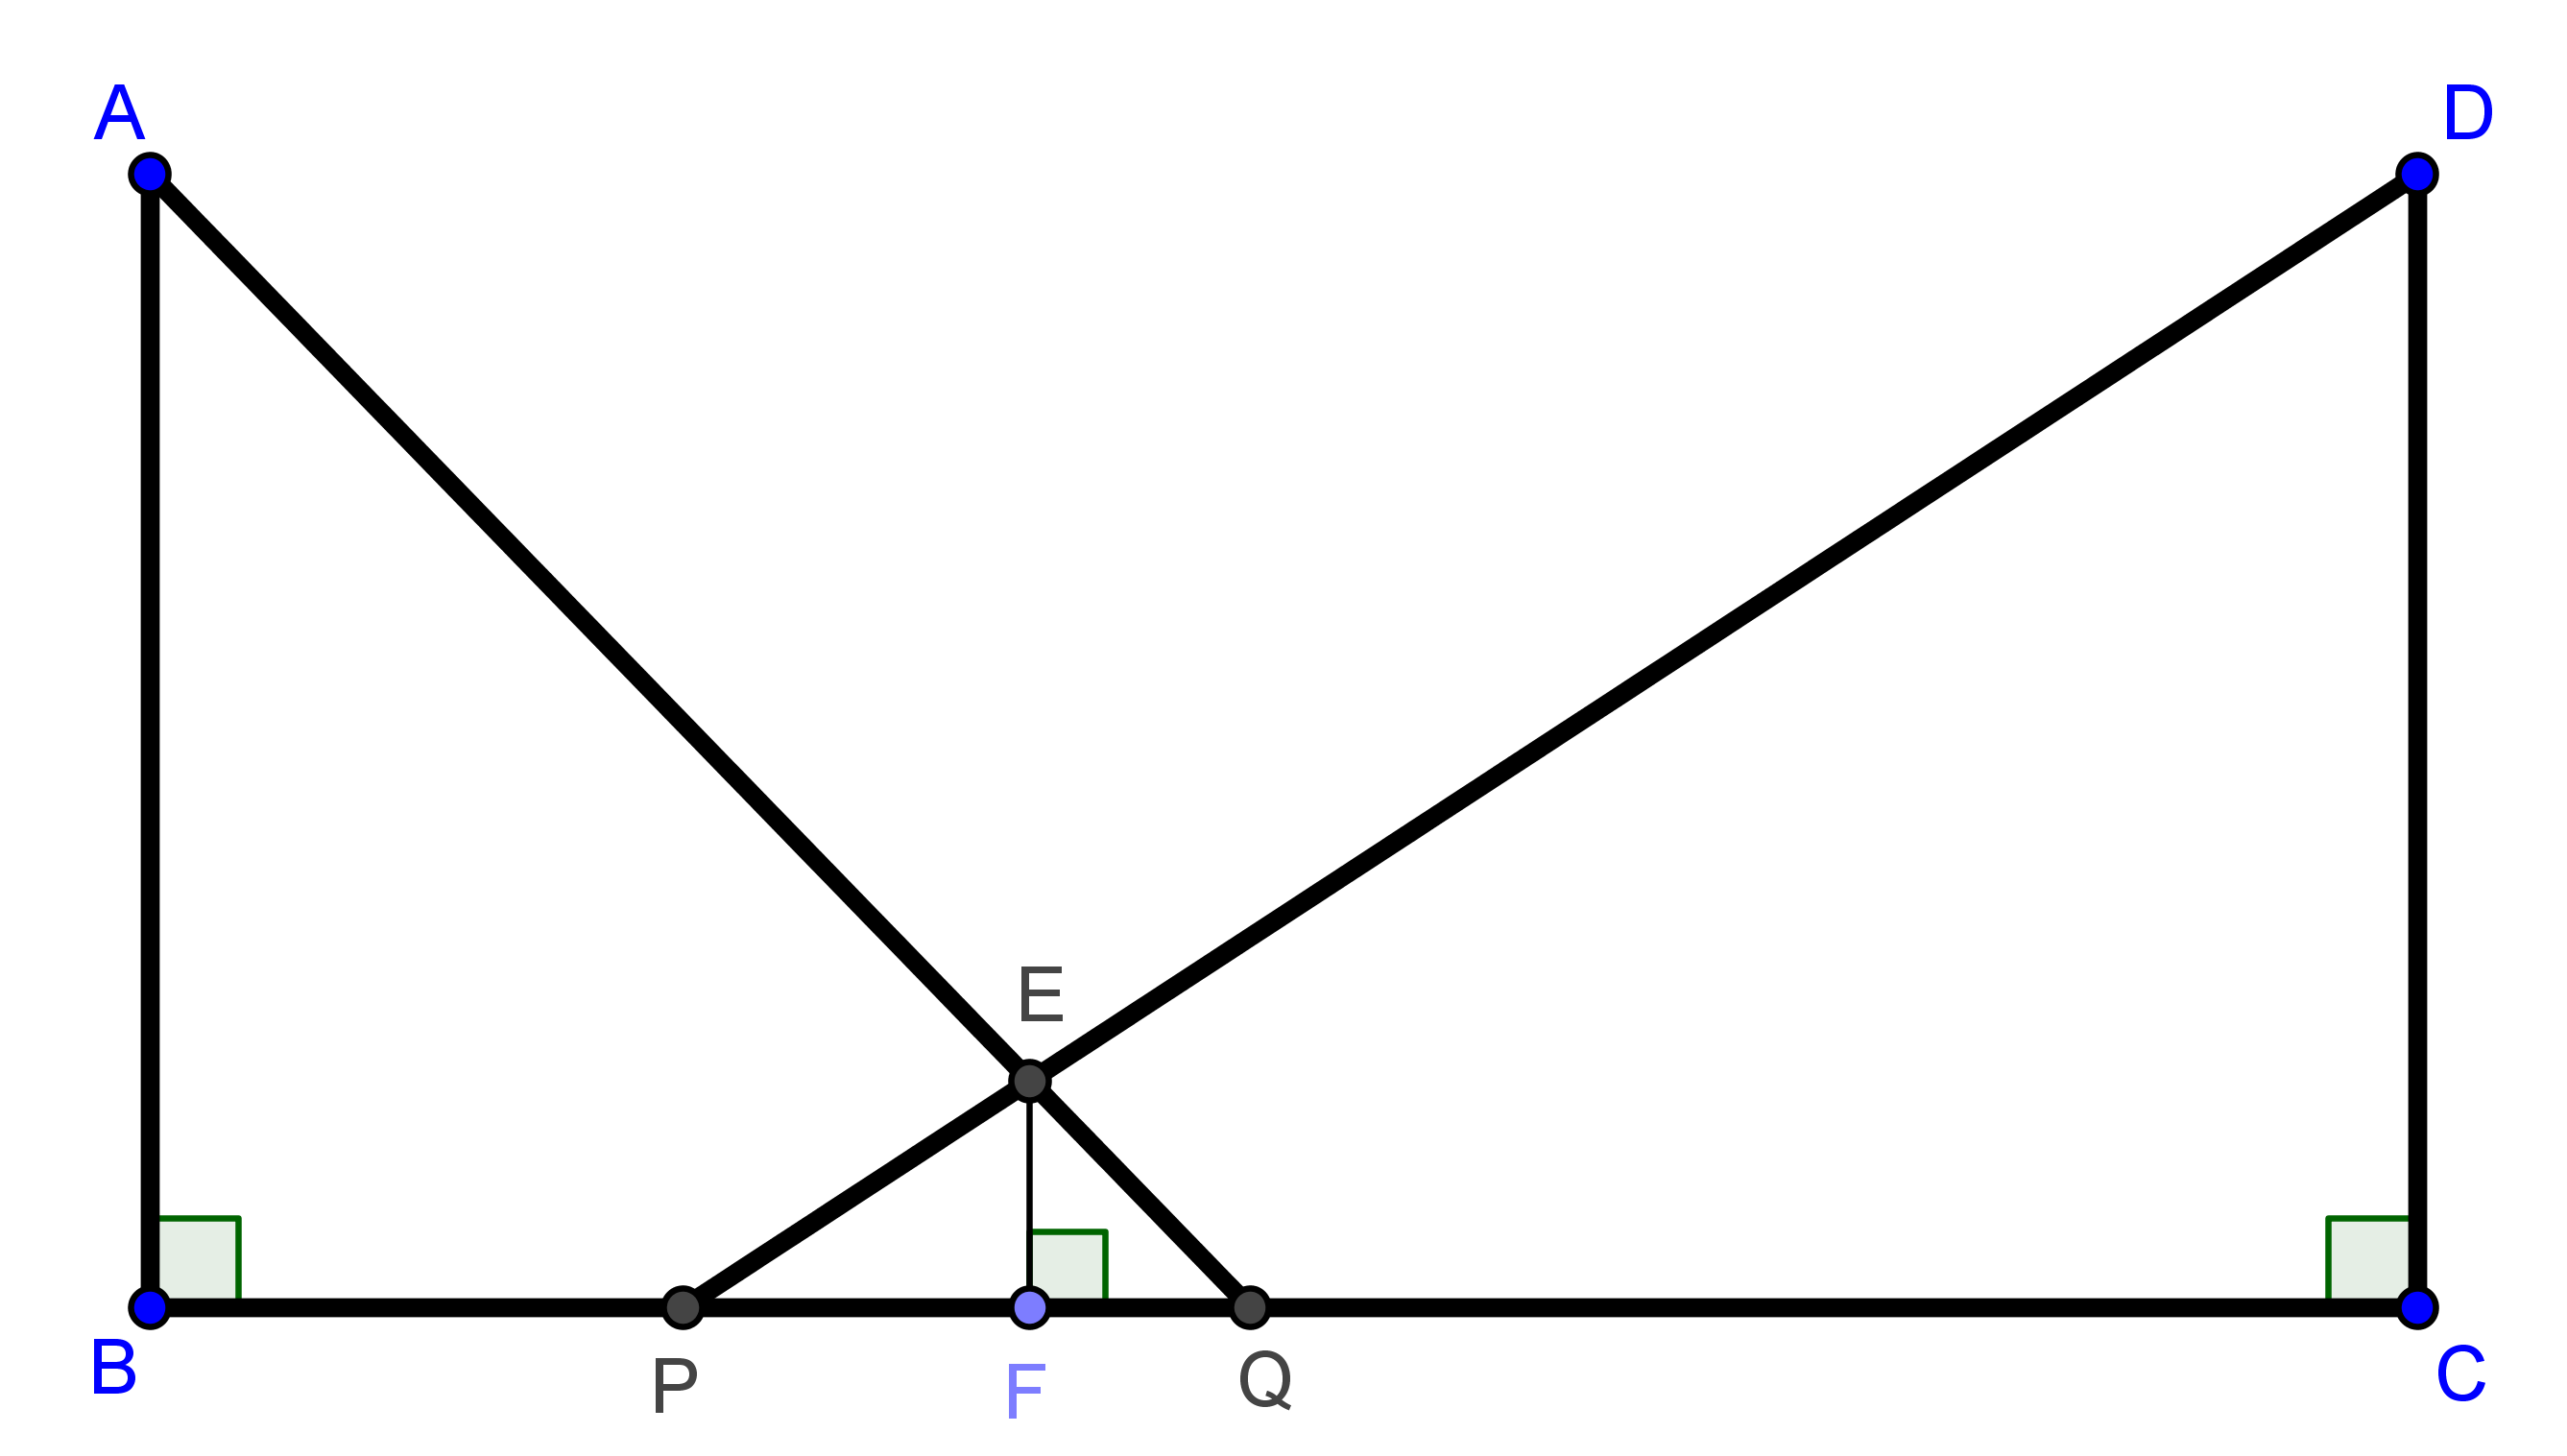
\includegraphics[width=0.5\textwidth]{top_math_p96_11}
\ep

\bp
\(\triangle EGH=10\)일 때, 평행사변형 \(\square ABCD\)의 넓이를 구하여라.
\par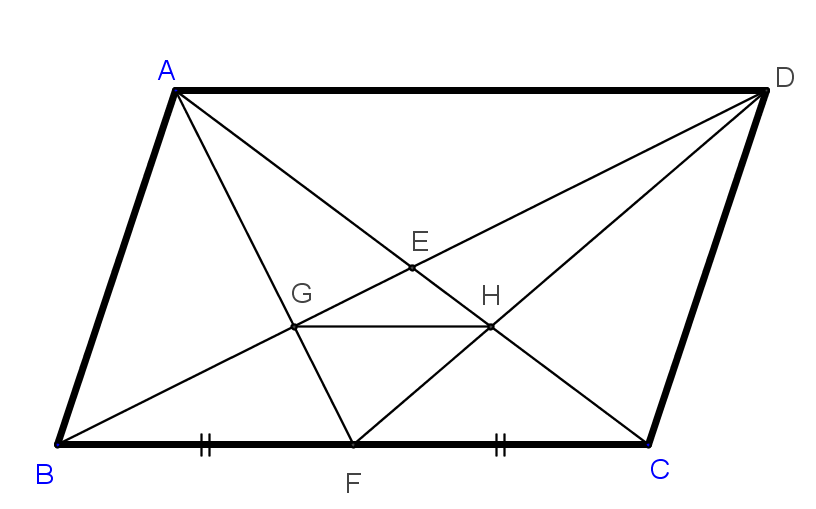
\includegraphics[width=0.5\textwidth]{top_math_p97_02}
\ep

\bp
\(\triangle DNE:\triangle ABD\)를 구하여라(\(BN=CN\)).
\par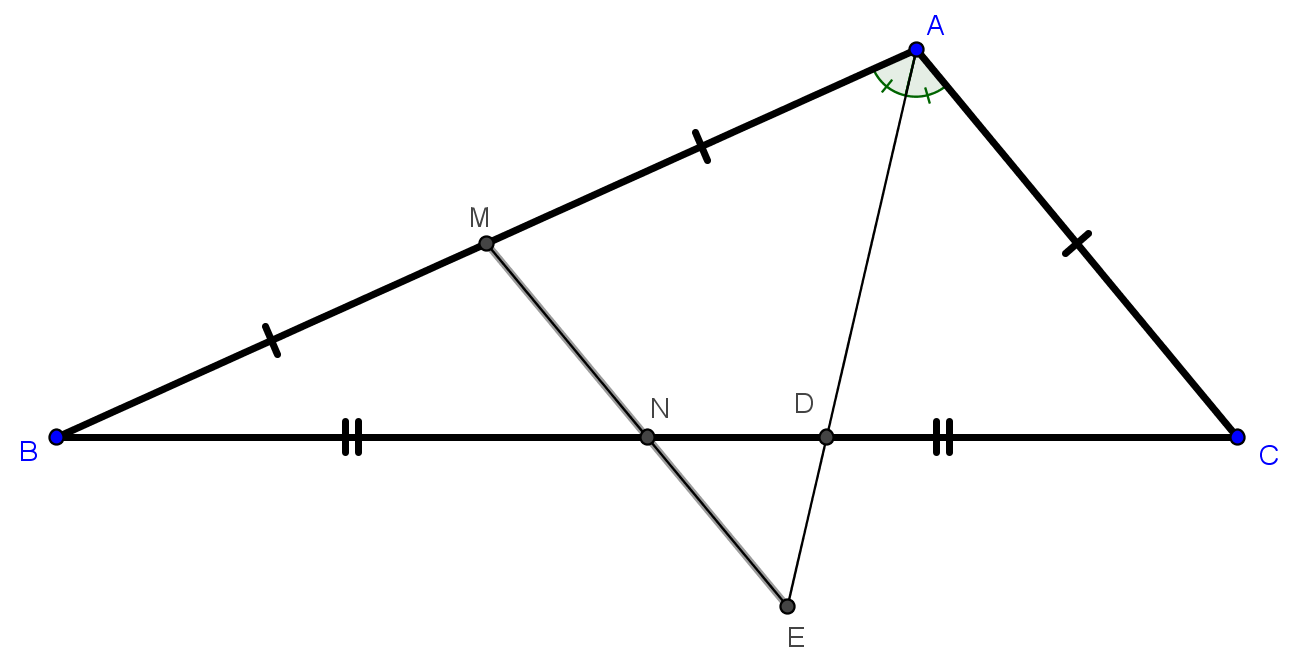
\includegraphics[width=0.5\textwidth]{top_math_p97_04}
\ep

\bp
\(AB=5\), \(BC=7\)일 때, \(\triangle ABC:\triangle ADE\)를 구하여라.
\par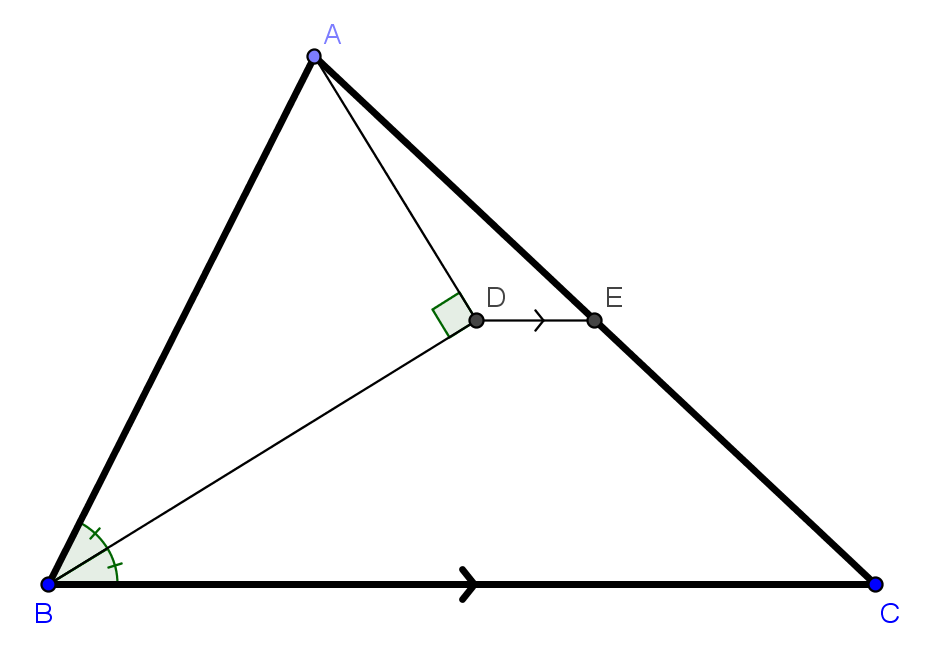
\includegraphics[width=0.5\textwidth]{top_math_p97_05}
\ep

\bp
\(AB=6\), \(AC=8\), \(AM=BM\)일 때, \(ME+MF\)를 구하여라.
\par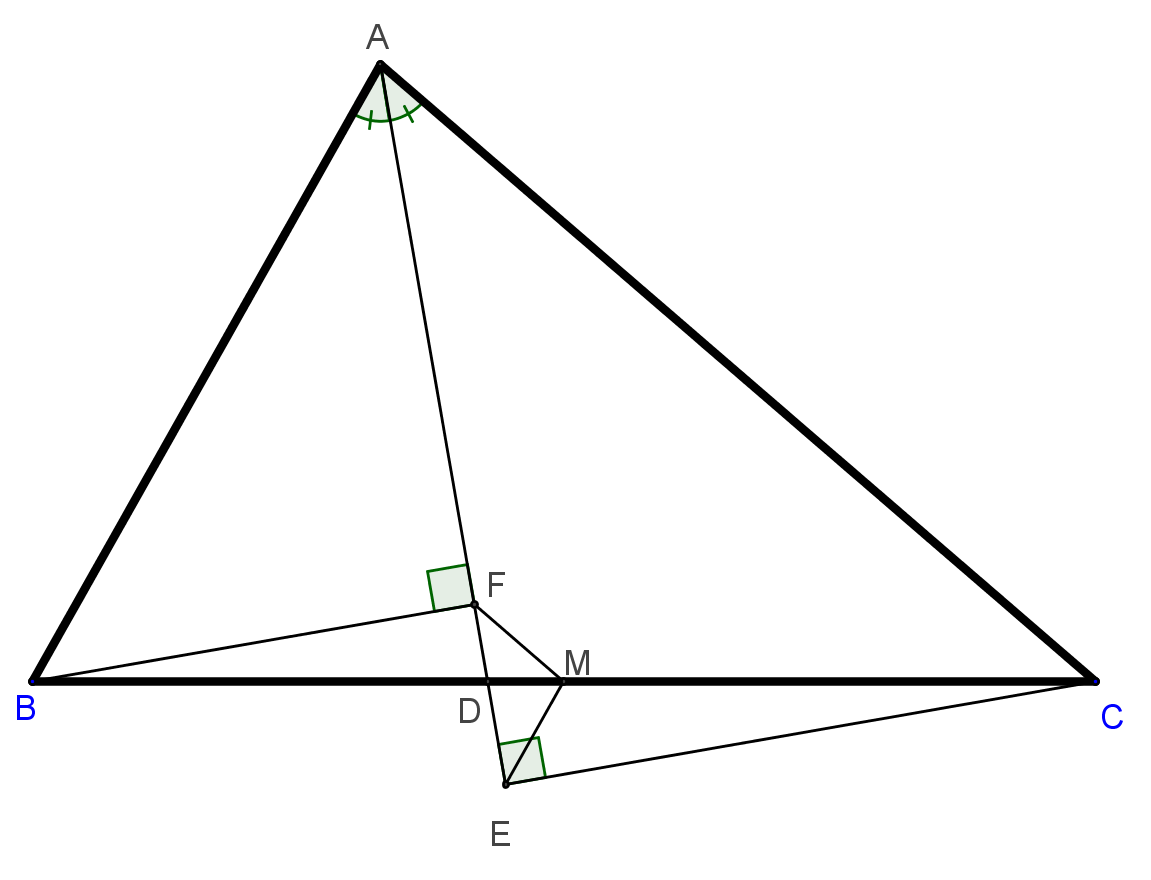
\includegraphics[width=0.5\textwidth]{top_math_p98_06}
\ep

\bp
\(BD=4\), \(CE=1\)이고 \(I\)는 \(\triangle ABC\)의 내심일 때, \(DE\)를 구하여라.
\par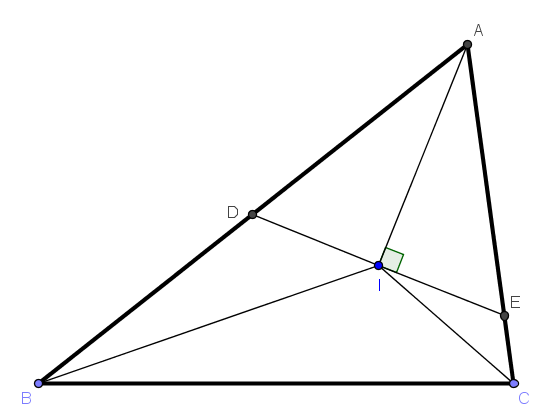
\includegraphics[width=0.5\textwidth]{top_math_p98_08}
\ep

\bp
\(\square ABCD\)는 평행사변형일 때,
\(\angle DFE\)의 크기를 구하여라.
\par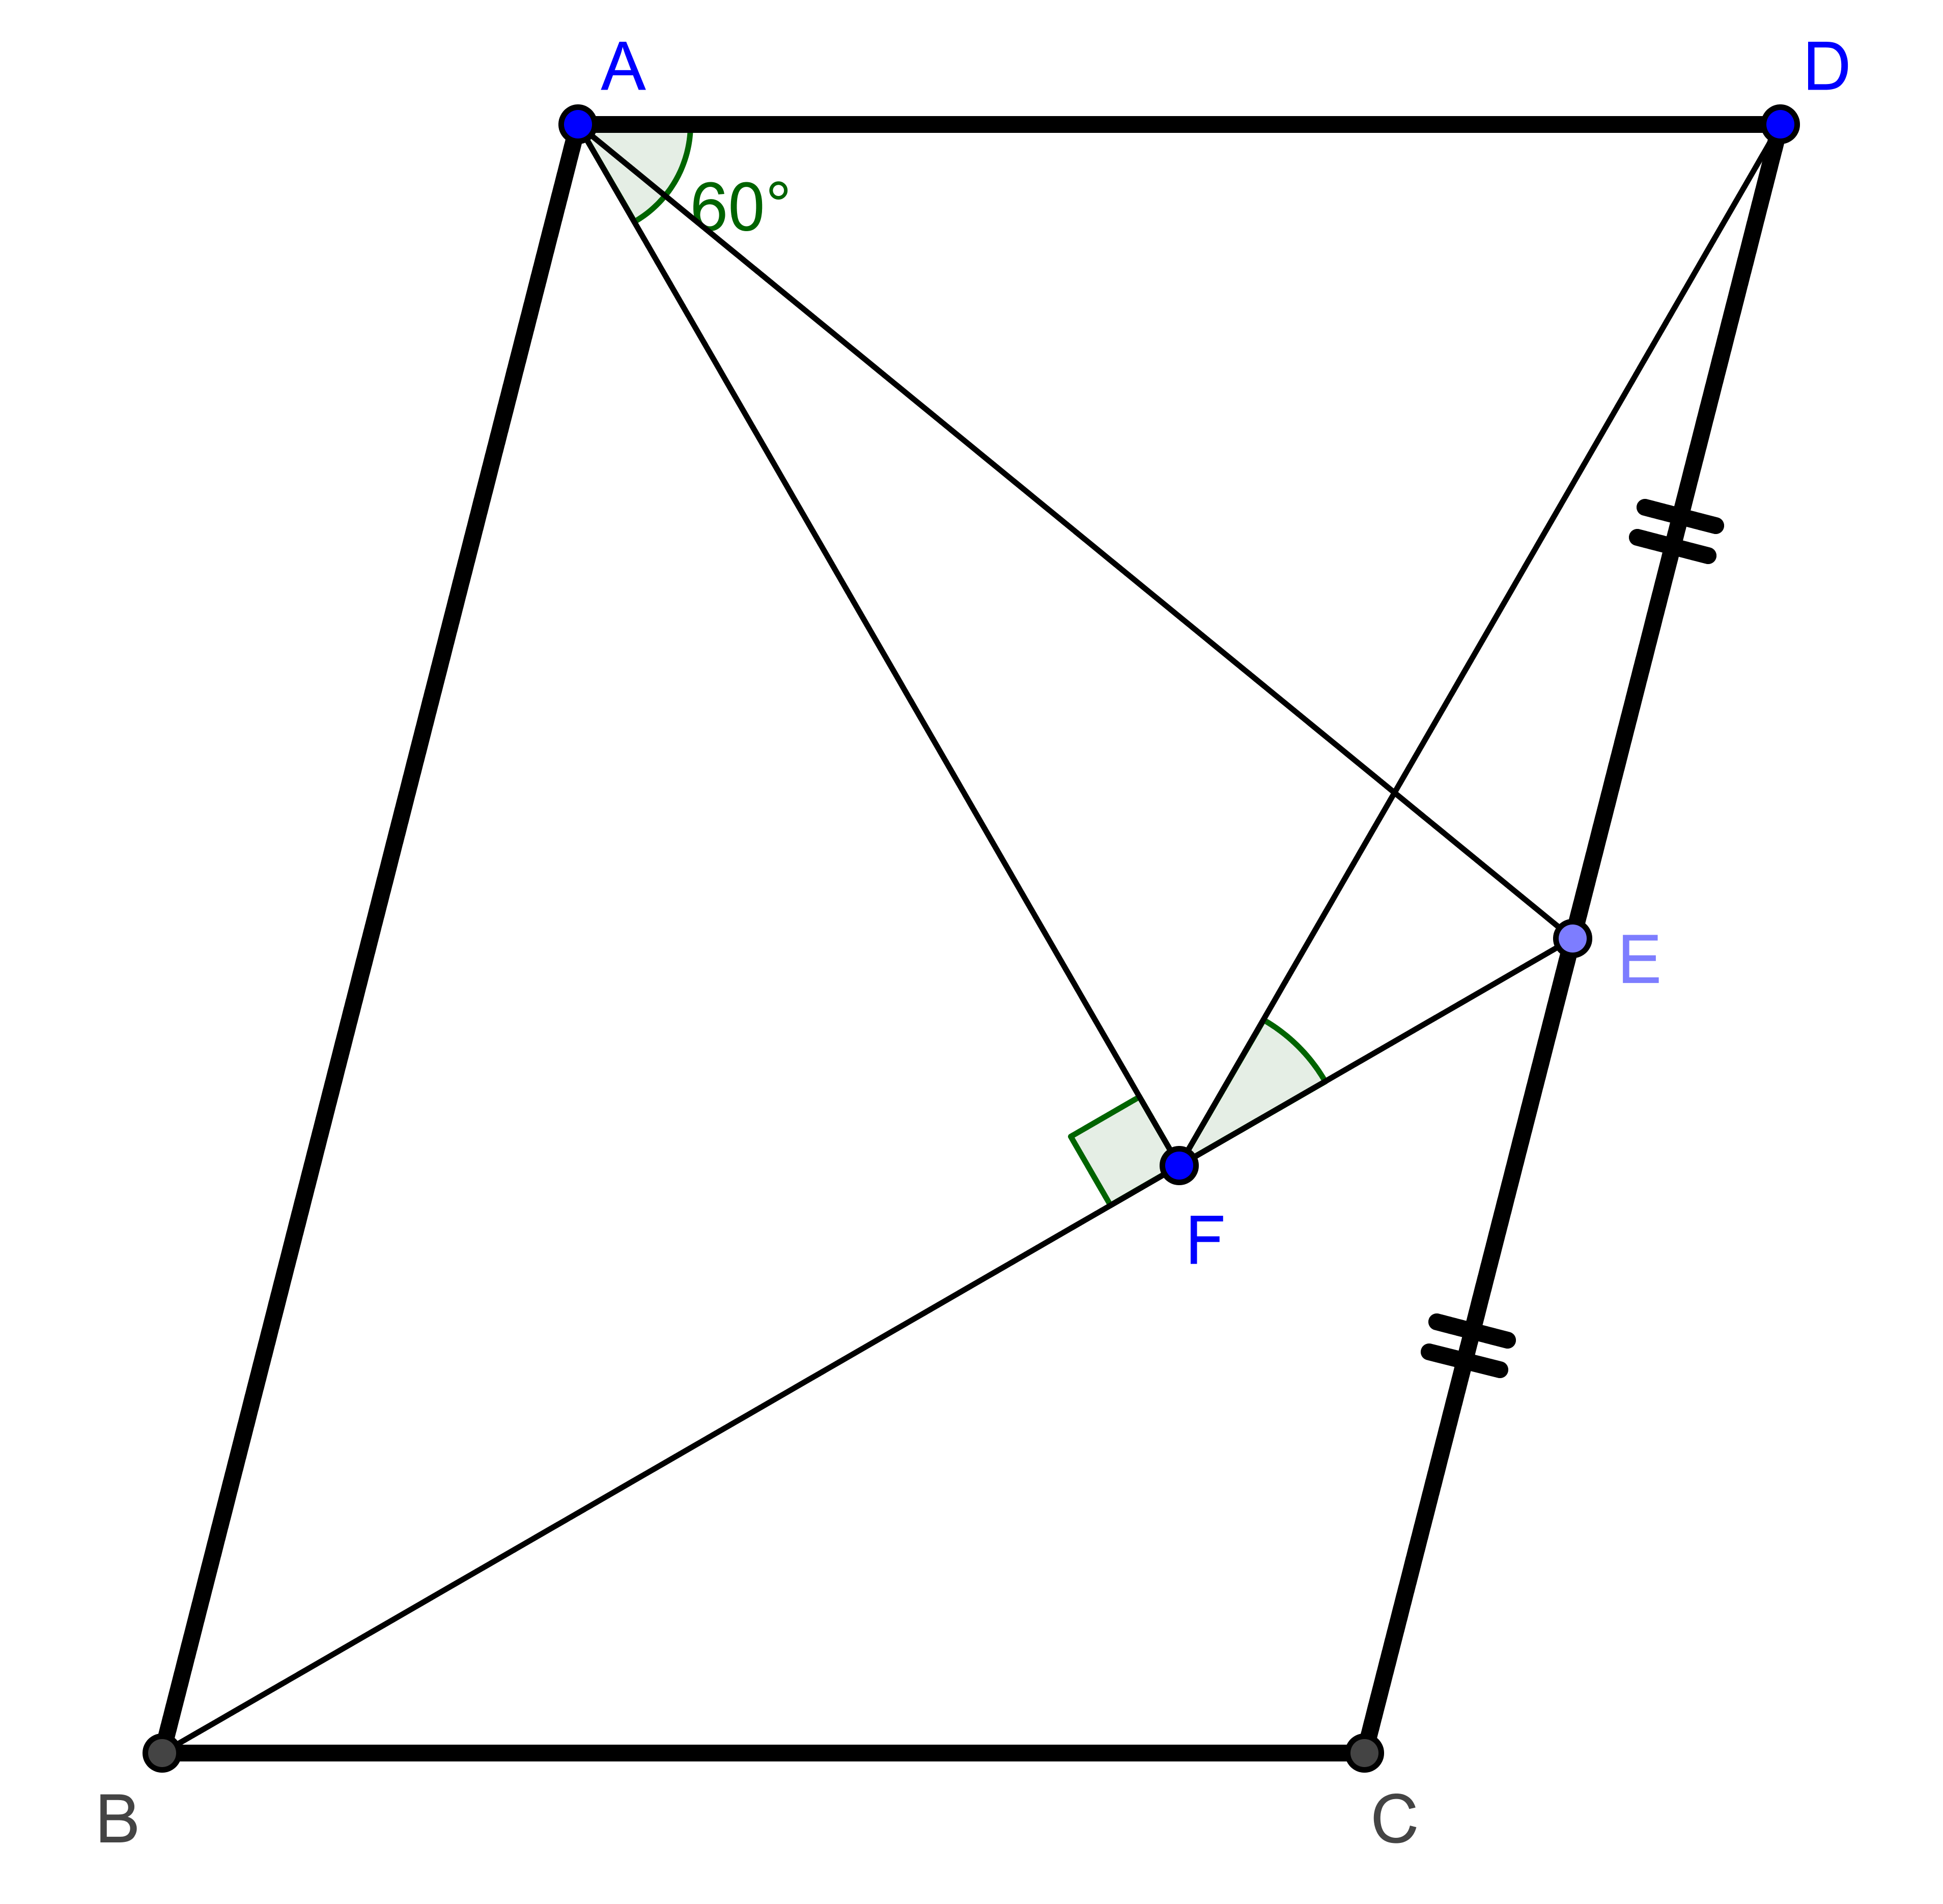
\includegraphics[width=0.5\textwidth]{top_math_p98_09}
\ep

\bp
\(AE=3\), \(ED=2\), \(BD=2\), \(DC=5\)일 때, \(\triangle ABE : \square CDEF\)를 구하여라.
\par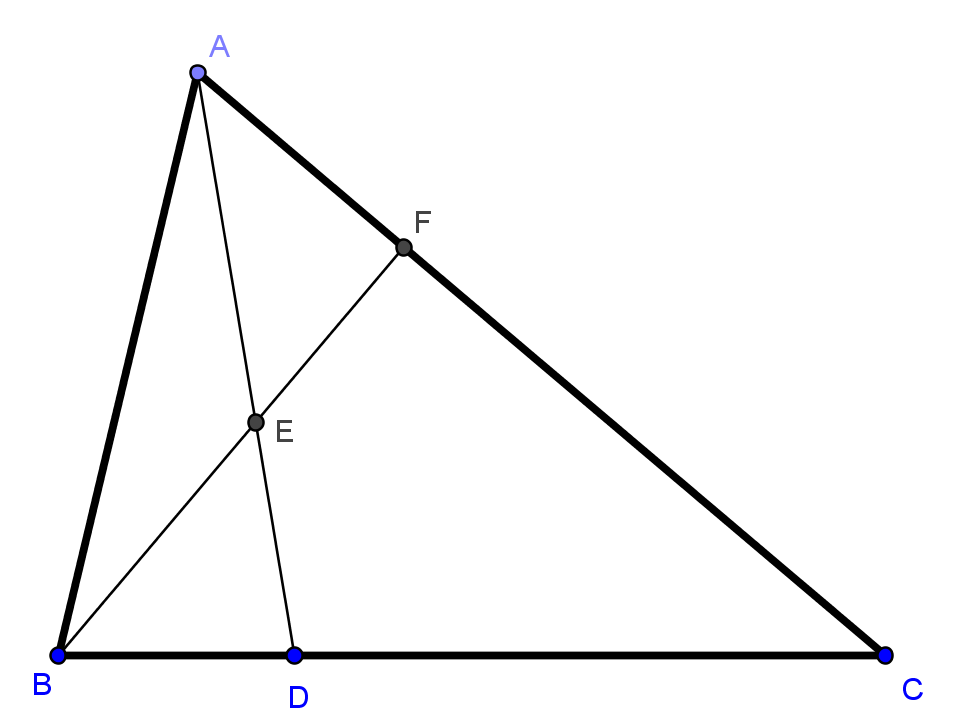
\includegraphics[width=0.5\textwidth]{top_math_p103_21}
\ep

\bp
\(AB=AC=12\)일 때, \(AE\)의 길이를 구하여라.
\par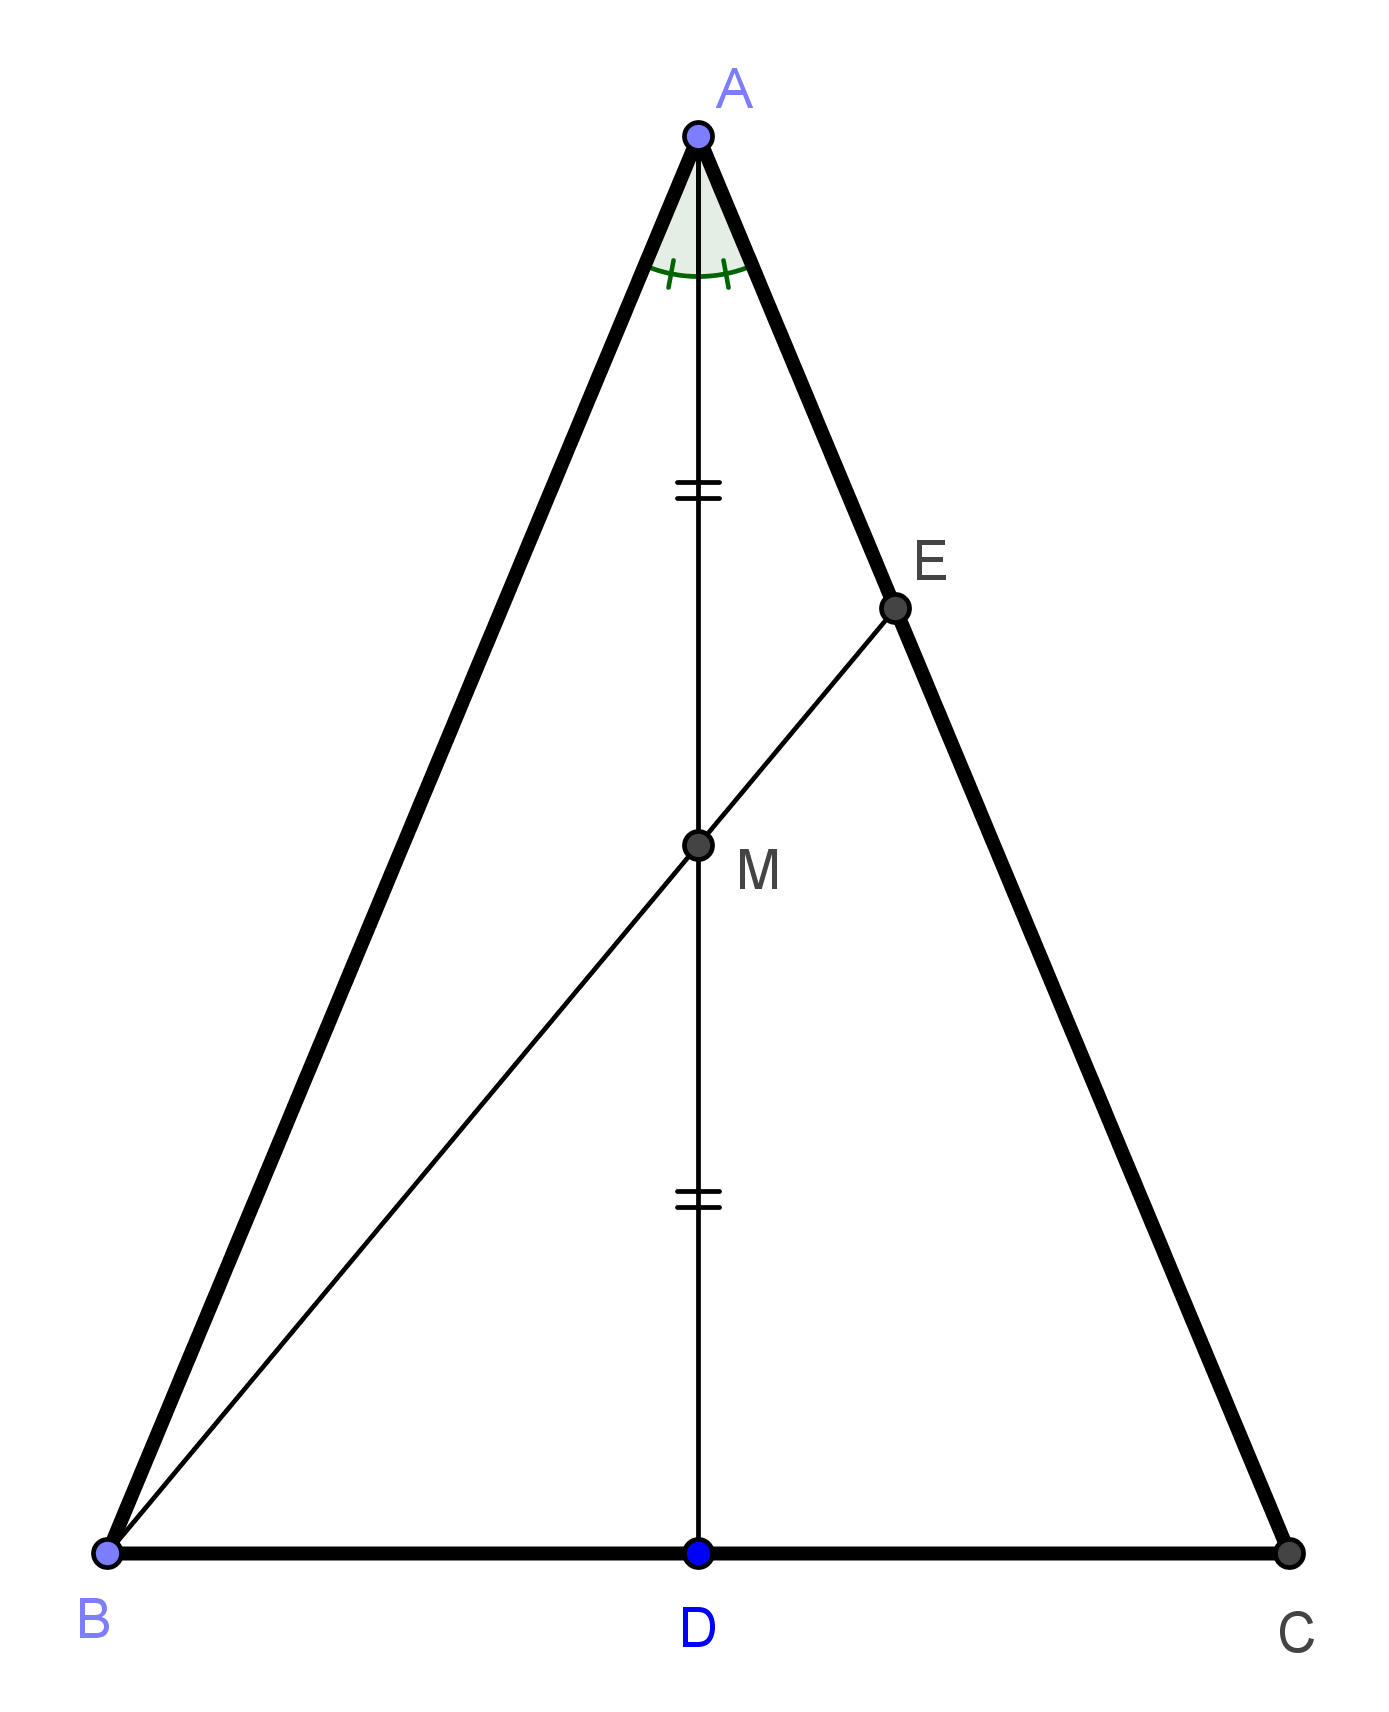
\includegraphics[width=0.5\textwidth]{top_math_p103_25}
\ep
\end{document}